% Consolidated equivalent of main.tex; edit either source form.
\documentclass[oneside,final,a4paper]{hcmut-report}

\usepackage{tabularx}
\usepackage{multirow}
\usepackage{tikz}
\usetikzlibrary{arrows.meta,positioning,matrix}
\setlength{\arrayrulewidth}{0.7pt}
\usepackage{microtype}
\setlength{\parindent}{0pt}
\setlength{\emergencystretch}{3em}
\setlength{\headheight}{44.3pt}
\captionsetup{labelfont=bf}



\deptname{Faculty of Computer Science and Engineering}
\coursename{Deep Learning and Its Applications (CO3133)}
\reporttype{ASSIGNMENT 1 -- FINAL REPORT}
\title{From Linear Models to Modern Sequence Models}
\advisor{Dr. Le Thanh Sach}
\groupname{Tiki-taka}
\reportplace{Ho Chi Minh City}
\reporttime{October, 2026}
\logofile{hcmut.png}

\newcommand{\classname}{CC01}
\newcommand{\instructorname}{Dr. Le Thanh Sach}
\newcommand{\groupinfo}{Tiki-taka}

% Cover layout adapted from the user-supplied OS_CAITOA template.
\newcommand{\bkcoverpage}{%
  \thispagestyle{empty}
  \begin{center}
    {\bfseries\fontsize{14}{16}\selectfont VIETNAM NATIONAL UNIVERSITY, HO CHI MINH CITY\par}
    \vspace{0.15cm}
    {\bfseries\fontsize{14}{16}\selectfont HO CHI MINH CITY UNIVERSITY OF TECHNOLOGY\par}
    \vspace{0.15cm}
    {\bfseries\fontsize{14}{16}\selectfont FACULTY OF COMPUTER SCIENCE AND ENGINEERING\par}
    \vspace{1.1cm}
    
\includegraphics[width=3.2cm]{hcmut.png}
    \vspace{0.9cm}

    {\bfseries\fontsize{17}{21}\selectfont DEEP LEARNING AND ITS APPLICATIONS\par}
    {\bfseries\fontsize{15}{19}\selectfont CO3133 -- SEMESTER-261\par}
    \vspace{0.5cm}
    {\bfseries\fontsize{16}{20}\selectfont ASSIGNMENT 1 -- FINAL REPORT\par}
    \vspace{0.45cm}
    {\bfseries\fontsize{20}{24}\selectfont
      From Linear Models to Modern Sequence Models:\par
      A Comparative Study for Image Classification\par}
    \vspace{0.9cm}

    \begin{tabular}{rl}
      \textbf{Class:} & \classname \\
      \textbf{Instructor:} & \instructorname \\
      \textbf{Group:} & \groupinfo \\
    \end{tabular}
    \vspace{0.35cm}

    \begin{tabular}{|c|l|c|}
      \hline
      \textbf{No.} & \textbf{Full Name} & \textbf{Student ID} \\
      \hline
      1 & Nguyen Anh Khoa & 2452539 \\ \hline
      2 & Nguyen Hao Thien & 2453194 \\ \hline
      3 & Ta Tuan Khai & 2452515 \\ \hline
    \end{tabular}
    \vfill
    {\bfseries Ho Chi Minh City, October, 2026}
  \end{center}
  \clearpage
}

\newcommand{\workdistributionpage}{%
  \thispagestyle{empty}
  \begin{center}
    {\bfseries\fontsize{17}{20}\selectfont WORK DISTRIBUTION}
  \end{center}
  \vspace{0.6cm}
  \noindent\textbf{Course:} Deep Learning and Its Applications -- CO3133\par
  \noindent\textbf{Assignment:} Assignment 1 -- Final Report\par
  \noindent\textbf{Class:} \classname\par
  \noindent\textbf{Instructor:} \instructorname\par
  \noindent\textbf{Group:} \groupinfo\par
  \vspace{0.7cm}
  \begin{center}
    \setlength{\tabcolsep}{4pt}
    \begin{tabularx}{\textwidth}{|c|>{\raggedright\arraybackslash}X|c|>{\raggedright\arraybackslash}X|c|}
      \hline
      \textbf{No.} & \textbf{Name} & \textbf{Student ID} & \textbf{Assigned Tasks} & \textbf{Completion} \\
      \hline
      1 & Nguyen Anh Khoa & 2452539 & Shared engine, MLP/GRU, metrics, checkpoints, and timing & 100\% \\ \hline
      2 & Nguyen Hao Thien & 2453194 & Dataset, EDA, preprocessing, Linear/CNN, and error analysis & 100\% \\ \hline
      3 & Ta Tuan Khai & 2452515 & Transformer, configurations, artifacts, integration, and report & 100\% \\ \hline
    \end{tabularx}
  \end{center}
  \clearpage
}


\usepackage[section]{placeins}
\usepackage{needspace}
\usepackage{xurl}
\newcolumntype{Y}{>{\raggedright\arraybackslash}X}
\makeatletter
\renewcommand\small{\@setfontsize\small{11pt}{13.2pt}}
\renewcommand\footnotesize{\@setfontsize\footnotesize{10pt}{12pt}}
\makeatother
\captionsetup{font=small,labelfont=bf}
\lstset{basicstyle=\ttfamily\footnotesize,breaklines=true,columns=fullflexible}
\setlength{\textfloatsep}{12pt plus 2pt minus 2pt}
\setlength{\floatsep}{10pt plus 2pt minus 2pt}
\setlength{\intextsep}{12pt plus 2pt minus 2pt}
\setcounter{topnumber}{3}
\setcounter{bottomnumber}{2}
\setcounter{totalnumber}{5}
\renewcommand{\topfraction}{.95}
\renewcommand{\bottomfraction}{.90}
\renewcommand{\textfraction}{.05}
\hypersetup{pdftitle={Tiki-taka A1 Final Report: Architecture Comparison on Fashion-MNIST},
pdfauthor={Nguyen Anh Khoa; Nguyen Hao Thien; Ta Tuan Khai}}

\begin{document}
\hypersetup{pageanchor=false}
\bkcoverpage
\workdistributionpage

\hypersetup{pageanchor=true}
\pagenumbering{roman}
\section*{Abstract}
\addcontentsline{toc}{section}{Abstract}
Across 15 Fashion-MNIST training runs, the custom Transformer achieves the highest
mean test accuracy and macro-F1, 91.267\% and 91.234\%, narrowly ahead of the
custom CNN at 90.690\% and 90.726\%.

The comparison uses five architecture families, one persisted stratified split and
three seeds per configuration. Selected checkpoints are evaluated on the official
10,000-image test source, with mean and sample standard deviation reported across seeds.

The CNN offers close predictive performance with about 72.9\% fewer parameters
than the Transformer and lower observed training-loop cost. Separately measured
Windows CPU inference favors different trade-offs; the model choice depends on
quality, size and the intended runtime.

All classifiers use shared preprocessing and metrics, while their representations
range from flattened pixels to spatial feature maps, image rows and patch tokens.
The study reports validation/test metrics, exact parameter counts, learning curves,
T4 train-and-validation loop times, explicitly labeled CPU timing, confusion
matrices and selected successes/failures. Shirt and related upper-body categories
remain difficult across models. Small seed count, different training policies and
separate timing environments prevent a causal or universal ranking of model families.
Effective configurations, run/checkpoint identities, verification records and
reconstruction instructions accompany the editable report source.

\clearpage
\tableofcontents
\clearpage

\pagenumbering{arabic}
\section{Problem and Data Description}
\label{sec:data}
\subsection{Problem Formulation and Research Questions}
Low-resolution product images provide a controlled setting for studying how model
structure affects classification. Fashion-MNIST includes visually similar garments,
so success requires distinguishing shape and texture rather than exploiting a class
frequency. We compare five implementations on a fixed partition and evaluation protocol.

Each input is a grayscale image \(X_i\in\mathbb{R}^{1\times28\times28}\) with one label
\(y_i\in\{0,\ldots,9\}\). A classifier produces ten raw scores:
\[
 f_\theta(X_i)=z_i\in\mathbb{R}^{10},\qquad
 \widehat y_i=\arg\max_{k\in\{0,\ldots,9\}} z_{i,k}.
\]
The objective is mean multiclass cross-entropy; probabilities are recorded for
interpretation, not supplied to the loss. The prediction unit is one image.
The comparison addresses four questions:
\begin{enumerate}
\item How do Linear, MLP, CNN, GRU and Transformer configurations compare in held-out
test accuracy and macro-F1?
\item How do flattened, spatial, row-sequence and patch-sequence representations relate
to their strengths and class-specific errors?
\item What trade-offs arise among predictive quality, parameter count, training cost
and measured CPU inference cost?
\item How much do results vary across training seeds 69420, 67 and 69?
\end{enumerate}
The results describe the tested configurations. Parameter count, optimization policy
and regularization also vary, so differences cannot be attributed solely to architecture.

\subsection{Dataset Description and Provenance}
Fashion-MNIST is the Zalando Research benchmark introduced by Xiao et al.\citep{fashion}
Its official sources contain 60,000 training and 10,000 test images, each an 8-bit
\(28\times28\) grayscale array, with ten labels and 7,000 examples per class across
both sources. The official repository publishes the dataset under the MIT
license.\citep{fashionlicense} Our loaders use
\texttt{torchvision.datasets.FashionMNIST} and the original IDX resources, without
changing the label mapping.

The original authors derive the benchmark from front-view catalog thumbnails.
Their conversion includes background-border trimming, subsampling, sharpening,
canvas centering, intensity inversion and grayscale conversion.\citep{fashion}
These are dataset-construction operations. The group starts from the distributed
IDX images and applies the separate transformations in Section~\ref{sec:preprocess}.
This distinguishes the dataset authors' processing from our code.

Raw IDX images have a 16-byte header and label files an 8-byte header.
Table~\ref{tab:inventory} records byte counts of the cached canonical resources used
for report verification. Each gzip resource was checked against the MD5 value in
torchvision's resource list, and decompression matched the IDX file byte-for-byte.
These are actual gzip sizes, rather than a generic archive-viewer size column.
\begin{table}[H]\centering\small
\caption{Verified canonical Fashion-MNIST resources in the local cache.}
\label{tab:inventory}
\begin{tabular}{lrr}
\toprule
Canonical resource & IDX bytes & Gzip bytes \\
\midrule
train-images images & 47,040,016 & 26,421,880 \\
train-labels labels & 60,008 & 29,515 \\
t10k-images images & 7,840,016 & 4,422,102 \\
t10k-labels labels & 10,008 & 5,148 \\
Total & 54,950,048 & 30,878,645 \\
\bottomrule
\end{tabular}

\end{table}
The four uncompressed IDX files occupy 54,950,048 bytes. This inventory describes
the cached resources; it does not assert an undocumented Kaggle acquisition session.

Limitations include small grayscale inputs, catalog-style backgrounds and overlapping
visual definitions among tops, shirts, pullovers and coats. Balanced label counts
do not remove content bias, annotation ambiguity or the domain gap from real photographs.

\subsection{Exploratory Data Analysis}
The saved stratified partition has exactly 5,000 training and 1,000 validation
examples per class; each official-test class also has 1,000 examples.
Table~\ref{tab:counts} was checked against the saved indices and raw labels.
The largest-to-smallest count ratio is 1.0 in each partition, so label imbalance
does not motivate resampling or class weighting here.
\begin{table}[H]\centering\small
\caption{Class support in the fixed seed-36 split.}
\label{tab:counts}
\begin{tabular}{rlrrr}
\toprule
ID & Class & Train & Validation & Test \\
\midrule
0 & T-shirt/top & 5000 & 1000 & 1000 \\
1 & Trouser & 5000 & 1000 & 1000 \\
2 & Pullover & 5000 & 1000 & 1000 \\
3 & Dress & 5000 & 1000 & 1000 \\
4 & Coat & 5000 & 1000 & 1000 \\
5 & Sandal & 5000 & 1000 & 1000 \\
6 & Shirt & 5000 & 1000 & 1000 \\
7 & Sneaker & 5000 & 1000 & 1000 \\
8 & Bag & 5000 & 1000 & 1000 \\
9 & Ankle boot & 5000 & 1000 & 1000 \\
\bottomrule
\end{tabular}

\end{table}

Figure~\ref{fig:representatives} shows the first four saved training indices of
each category. These are unaugmented training images, not examples chosen using
test performance. Their variation and shared upper-body silhouettes suggest
plausible sources of confusion.
\begin{figure}[H]\centering
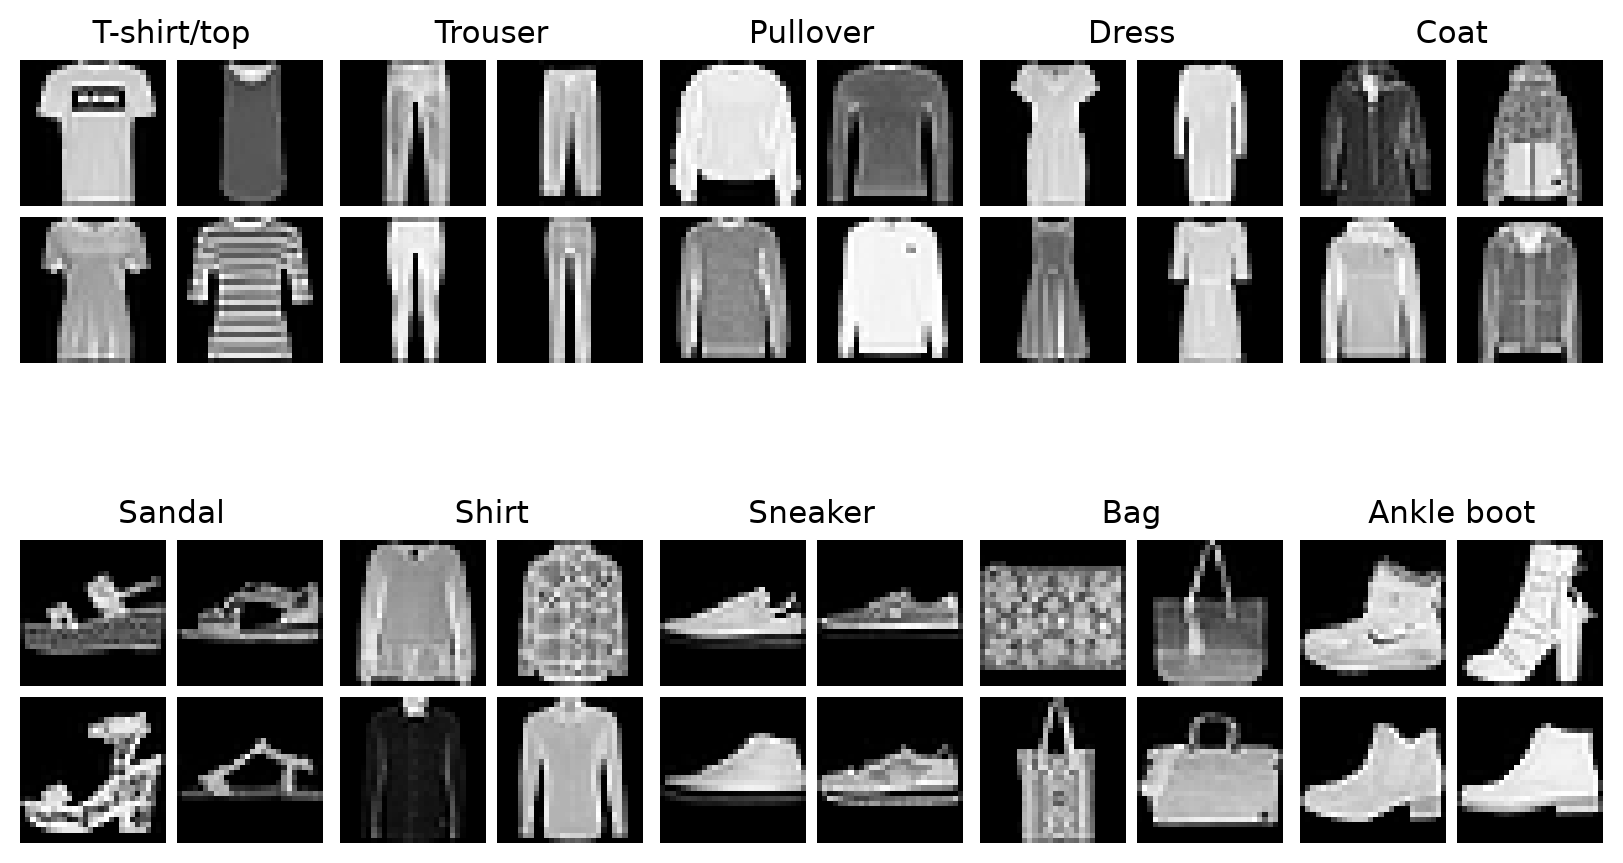
\includegraphics[width=\linewidth]{figures/training_examples.png}
\caption{Forty representative training images: four examples per class panel.
Selection IDs are retained in \texttt{evidence/eda\_selection.json}.}
\label{fig:representatives}
\end{figure}
Visual similarity alone does not establish prediction confidence. Actual probabilities
and confusion frequencies are examined in Sections~\ref{sec:confusion}
and~\ref{sec:qualitative}. No manual relabeling, perceptual duplicate removal or
custom outlier filtering was performed.

\subsection{Data Splitting and Leakage Prevention}
The official training source is stratified into 50,000 training and 10,000 validation
images with split seed 36. The official 10,000-example test source remains separate.
The persisted manifest is \path{configs/a1/splits/fashion_mnist_split.json};
ordinary loader construction reads it instead of resampling a new split.

The validator checks index ranges, duplicates, full source coverage and disjoint
training/validation membership. Test indices use a different source namespace even
when their integer values coincide with training indices. Normalization is fitted
on unaugmented training indices only. Validation selects checkpoints; final test
scores do not select a checkpoint or the best seed.

The short excerpt below uses the implementation's actual manifest fields:
\begin{lstlisting}[style=pythoncode]
train_indices = manifest.train_indices
val_indices = manifest.validation_indices
test_indices = manifest.test_indices
\end{lstlisting}
These controls prevent index overlap and normalization leakage. They do not establish
that visually duplicated product images have been removed across partitions;
no perceptual-duplicate audit is claimed.

\subsection{Preprocessing, Augmentation and Example Batch}
\label{sec:preprocess}
All five main configurations use the same training-only random crop:
\(28\times28\) output after two pixels of zero-valued constant padding per side.
No horizontal flip is enabled. Tensor conversion scales uint8 pixels to \([0,1]\),
then applies the training-derived statistics:
\[
 \mu=0.28585961086061534,\qquad
 \sigma=0.352790375749525,\qquad x'=(x-\mu)/\sigma.
\]
Validation and test apply tensor conversion and this normalization without random
augmentation. Their values do not contribute to fitting the statistics.

Every reported main run has configured batch size 64 and retains the last incomplete
batch. The shared contract is float32 images \([B,1,28,28]\), int64 labels \([B]\),
and \(B\) stable sample IDs. For instance,
\texttt{fashion\_mnist:official\_test:0} identifies an original test image, not a
batch-relative position.

Figure~\ref{fig:batch} shows six entries of a 64-example batch regenerated for the
report from saved training indices, using crop RNG seed 69420 and the same transform
definition. This is a post-hoc data illustration, not a logged training-epoch batch.
Its actual shape is \([64,1,28,28]\), dtype float32, and observed normalized range
approximately \([-0.8103,2.0243]\). The display maps that fixed range to grayscale.
\begin{figure}[H]\centering
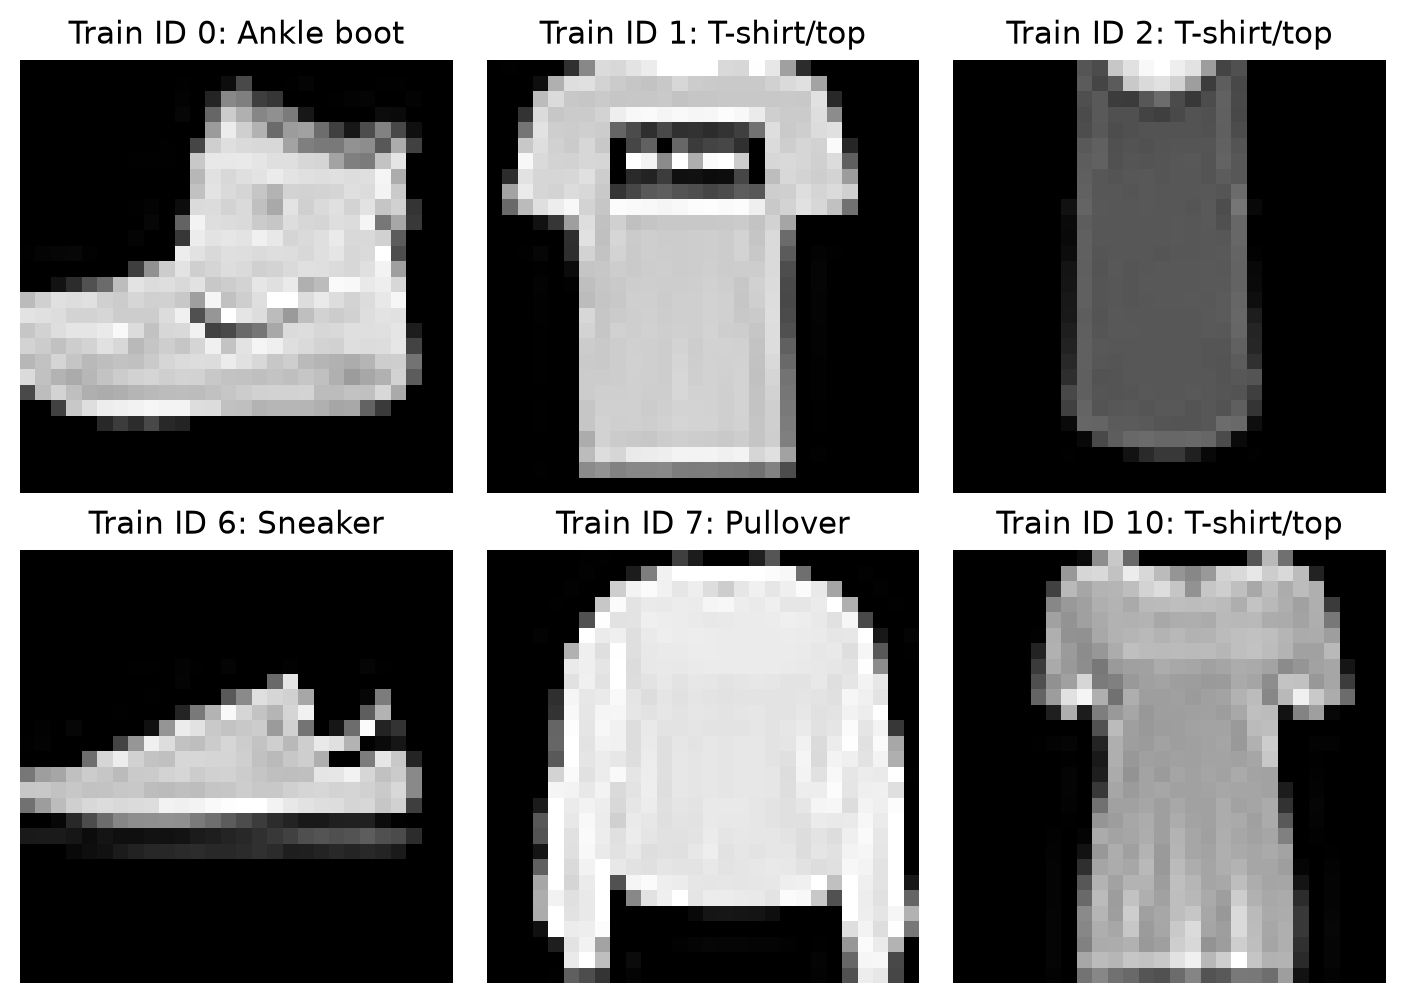
\includegraphics[width=.90\linewidth]{figures/preprocessed_batch.png}
\caption{Post-hoc example training batch after crop and normalization. Six of 64
images are shown; IDs/statistics are saved in \texttt{evidence/example\_batch.json}.}
\label{fig:batch}
\end{figure}
\FloatBarrier

\clearpage
\section{Methodology}
\label{sec:methods}
\subsection{End-to-End Pipeline and Data Loading}
The pipeline uses a custom subset wrapper and collation function around torchvision's
raw Fashion-MNIST dataset. Training and validation wrappers use disjoint official-training
indices and independent transform objects; the test wrapper uses the official test
source. Training shuffles through a dedicated run-seeded generator. Validation and
test do not shuffle. All loaders retain IDs and use \texttt{drop\_last=False}.

Figure~\ref{fig:pipeline} separates the update and evaluation paths. Training enables
dropout and gradients; validation/test use evaluation mode and inference without
gradient tracking. Both consume the same image/label batch contract.
\begin{figure}[H]\centering
\begin{tikzpicture}[>=Latex,node distance=8mm and 9mm,
 box/.style={draw,rounded corners,align=center,text width=39mm,minimum height=12mm,
 font=\small,fill=blue!5}]
\node[box] (raw) {Raw IDX + fixed\\split manifest};
\node[box,right=of raw] (prep) {Train crop / eval\\tensor + normalization};
\node[box,right=of prep] (loader) {DataLoader\\images, labels, IDs};
\node[box,below=of prep] (model) {Model forward\\raw logits \([B,10]\)};
\node[box,below left=of model,fill=orange!10] (loss) {Cross-entropy\\backward + Adam};
\node[box,below right=of model,fill=green!8] (eval) {Argmax + probabilities\\metrics + saved outputs};
\draw[->] (raw)--(prep); \draw[->] (prep)--(loader);
\draw[->] (loader.south)|-(model.east);
\draw[->] (model.south west)--node[midway,above left,font=\small]{train} (loss.north east);
\draw[->] (model)--node[above right,font=\small]{evaluate} (eval);
\draw[->,dashed] (loss.west)-|([xshift=-5mm]raw.west)|-
node[pos=.8,above,font=\small]{parameter update} (model.west);
\end{tikzpicture}
\caption{Data preparation and model interface, with distinct update/evaluation paths.
Softmax probabilities support analysis; cross-entropy receives raw logits.}
\label{fig:pipeline}
\end{figure}
The engine computes sample-weighted loss and epoch-level accuracy/F1 from online
training predictions. These include augmentation and training-mode behavior.
Thus, close train/validation curves alone do not prove absence of overfitting.

\subsection{Shared Model Interface and Input Representations}
Every classifier accepts float32 \([B,1,28,28]\) and returns raw \([B,10]\) logits.
Representation changes occur inside the model, leaving data loading and metrics
unchanged. Table~\ref{tab:representations} connects each representation to its
structural preference.
\begin{table}[H]\centering\small
\caption{Representations used in the reported configurations.}
\label{tab:representations}
\begin{tabularx}{\linewidth}{lYY}
\toprule Model & Internal representation & Structural preference\\\midrule
Linear & Flattened 784-vector & One affine decision rule per class\\
MLP & Flattened vector, dense hidden features & Nonlinear global combinations\\
CNN & Two-dimensional feature maps & Local connectivity and shared filters\\
GRU & 28 row timesteps of width 28 & Ordered recurrent context\\
Transformer & 49 \(4\times4\) patches, width 64 & Position-aware token interactions\\
\bottomrule
\end{tabularx}
\end{table}
The input shape and label space are shared despite different learned representations
and parameter counts.

\subsection{Model Architectures}
\subsubsection{Linear / Softmax Classifier}
The baseline flattens each image and applies one affine layer:
\[
 x=\operatorname{flatten}(X)\in\mathbb{R}^{784},\qquad
 z=Wx+b,\quad W\in\mathbb{R}^{10\times784}.
\]
There is no hidden nonlinearity. The \(784\times10+10=7,850\) parameters are all
trainable; flattening adds none. Probabilities, when needed, are
\(p_k=\exp(z_k)/\sum_{j=0}^{9}\exp(z_j)\).
The implementation returns logits because cross-entropy already combines
log-softmax and the label loss.\citep{pytorchce}
The project implements the wrapper and validation around PyTorch
\texttt{nn.Flatten} and \texttt{nn.Linear}. This small baseline has neither
a hidden feature hierarchy nor built-in image locality.

\subsubsection{Multilayer Perceptron}
The MLP uses \(784\rightarrow256\rightarrow128\rightarrow10\).
Every hidden affine layer is followed by ReLU and dropout 0.1; the final layer
returns logits. For hidden layer \(\ell\),
\[
 a_\ell=W_\ell h_{\ell-1}+b_\ell,\qquad
 h_\ell=\operatorname{ReLU}(a_\ell).
\]
ReLU keeps positive values and sets negative values to zero, enabling nonlinear
boundaries. Without nonlinearities, consecutive affine layers collapse into one
affine transformation. Training-time dropout masks hidden activations and scales
retained values; evaluation disables these masks. It regularizes dense features,
but does not favor spatially adjacent pixels.
The parameter count is
\[
 (784\cdot256+256)+(256\cdot128+128)+(128\cdot10+10)=235,146.
\]
Project code assembles the network from PyTorch layers. Other activation names
are supported, but only ReLU is used in the reported MLP runs; no activation
ablation is claimed.

\subsubsection{Custom Convolutional Neural Network}
Convolutions apply learned filters to local neighborhoods, reusing weights across
positions. Multiple filters yield feature maps responsive to patterns learned
from data. For stride one, a filter response has the form
\[
 Z_{m,i,j}=b_m+\sum_c\sum_u\sum_v W_{m,c,u,v}X_{c,i+u,j+v}.
\]
For illustration, a \(2\times2\) filter with ones on its main diagonal gives
\(1+6=7\) on \(\bigl[\begin{smallmatrix}1&2\\5&6\end{smallmatrix}\bigr]\).
This is a numerical example; the actual network uses \(3\times3\) kernels.

Max pooling retains the largest value in a region: the same example pools to 6,
versus 3.5 under average pooling. Pooling reduces spatial resolution and may reduce
sensitivity to small shifts, while discarding fine spatial detail. Its aggregation
rule has no trainable weights.

Table~\ref{tab:cnn} gives the actual custom architecture. Padding preserves each
convolution's size; max pooling reduces spatial dimensions \(28\to14\to7\).
The implementation uses \texttt{ceil\_mode=True}; these even-sized inputs have
the dimensions shown. Adaptive average pooling gives one value per channel.
\begin{table}[H]\centering\small
\caption{Custom CNN layers and resulting tensor shapes.}
\label{tab:cnn}
\begin{tabular}{ll}
\toprule Layer & Output\\\midrule
Input & \([B,1,28,28]\)\\
Conv \(1\to32\), \(3\times3\), pad 1; ReLU & \([B,32,28,28]\)\\
MaxPool \(2\times2\) & \([B,32,14,14]\)\\
Conv \(32\to64\), \(3\times3\), pad 1; ReLU & \([B,64,14,14]\)\\
MaxPool \(2\times2\) & \([B,64,7,7]\)\\
AdaptiveAvgPool; flatten & \([B,64]\)\\
Linear \(64\to128\); ReLU; Dropout 0.1 & \([B,128]\)\\
Linear \(128\to10\) & \([B,10]\)\\\bottomrule
\end{tabular}
\end{table}
All 28,426 parameters are trainable. The project defines this network using
PyTorch convolution, activation, pooling and linear layers; it is not a pretrained
CNN backbone.

\subsubsection{GRU-Based Image Classifier}
Each image row is one timestep,
\[
 x_t=X_{t,:}\in\mathbb{R}^{28},\qquad t=1,\ldots,28.
\]
The batch-first sequence has shape \([B,28,28]\). A single unidirectional
\texttt{nn.GRU} uses input width 28 and hidden width 128; its final hidden
state is projected to ten logits. A timestep is a complete row, not one pixel.
The traversal carries information from earlier rows into later decisions.

The equations below match the PyTorch cell actually used:\citep{pytorchgru}
\begin{align*}
 r_t&=\sigma(W_{ir}x_t+b_{ir}+W_{hr}h_{t-1}+b_{hr}),\\
 z_t&=\sigma(W_{iz}x_t+b_{iz}+W_{hz}h_{t-1}+b_{hz}),\\
 n_t&=\tanh(W_{in}x_t+b_{in}+r_t\odot(W_{hn}h_{t-1}+b_{hn})),\\
 h_t&=(1-z_t)\odot n_t+z_t\odot h_{t-1}.
\end{align*}
The reset gate modulates transformed past information in the candidate; the update
gate blends it with retained memory. PyTorch multiplies by the reset gate after
the hidden affine transformation.

Recurrent weights and two bias vectors contribute
\(3(28\cdot128+128\cdot128+2\cdot128)=60,672\) parameters.
The head adds 1,290, totaling 61,962. The project wrapper handles row conversion
and state selection, while the cell is a PyTorch component. Although the code
supports columns, LSTM and bidirectionality, these variants were not evaluated.
The reported single-layer GRU has no inter-layer dropout transition.

\subsubsection{Custom Transformer Classifier}
The custom Transformer divides an image into a \(7\times7\) grid of
non-overlapping \(4\times4\) patches. The 49 patches are flattened to 16 values
each and projected to embedding width 64. A learned \(49\times64\) position
embedding is added:
\[
 P\in\mathbb{R}^{B\times49\times16},\qquad
 H_0=PW_E+b_E+E_{\rm pos}\in\mathbb{R}^{B\times49\times64}.
\]
This represents local regions as tokens while preserving their image positions.
Two pre-normalized residual blocks contain four-head self-attention and an FFN.
Each head has \(d_h=16\):
\[
 Q=HW_Q,\quad K=HW_K,\quad V=HW_V,\qquad
 A=\operatorname{softmax}\!\left(QK^\mathsf{T}/\sqrt{16}\right)V.
\]
Per image, attention weights have shape \([4,49,49]\). Each token attends to all
49 tokens and receives a 16-value result per head; concatenation and an output
projection restore width 64. The mechanism follows scaled dot-product
attention,\citep{attention} with the project's residual structure
\begin{align*}
 U_\ell&=H_{\ell-1}+
 \operatorname{Dropout}\bigl(\operatorname{MHSA}(\operatorname{LN}(H_{\ell-1}))\bigr),\\
 H_\ell&=U_\ell+\operatorname{FFN}(\operatorname{LN}(U_\ell)).
\end{align*}
The FFN is \(64\to256\to64\), with GELU and dropout 0.1. After two blocks,
final layer normalization and mean pooling over 49 tokens give a 64-value vector;
a \(64\to10\) head returns logits. There is no class token.

Parameter counts are 1,088 for patch projection, 3,136 for positions,
two blocks of 49,984, 128 for final normalization and 650 for the head:
104,970 in total. The project implements patchification, Q/K/V projections,
attention, residual blocks and pooling with PyTorch tensor operations and layers.
It does not substitute a built-in Transformer encoder or pretrained vision model.
\FloatBarrier

\subsection{Loss Function and Evaluation Metrics}
Every model uses unweighted multiclass cross-entropy:
\[
 L=-\frac{1}{N}\sum_{i=1}^{N}
 \log\frac{\exp(z_{i,y_i})}{\sum_{k=0}^{9}\exp(z_{i,k})}.
\]
Loss is aggregated by sample count, correctly weighting the incomplete final
batch. Argmax logits give labels. For a confusion matrix whose rows are true
classes and columns predictions,
\[
 \mathrm{Accuracy}=\frac{\sum_c C_{cc}}{\sum_{c,k}C_{ck}},\qquad
 P_c=\frac{TP_c}{TP_c+FP_c},\quad R_c=\frac{TP_c}{TP_c+FN_c},
\]
\[
 F1_c=\frac{2P_cR_c}{P_c+R_c},\qquad
 \mathrm{MacroF1}=\frac{1}{10}\sum_{c=0}^{9}F1_c.
\]
Undefined class precision, recall or F1 is assigned zero, matching
\texttt{zero\_division=0}. Macro-F1 weights classes equally and can reveal
weaknesses hidden by overall accuracy. Tables use the mean and sample SD across
three training seeds, with denominator \(n-1\). Scores converted to percent are
labeled explicitly; differences between percent scores are percentage points.

\subsection{Training, Hyperparameter Selection and Checkpointing}
\label{sec:training}
All 15 main runs use Adam, learning rate \(10^{-3}\), weight decay 0, batch size
64 and a 100-epoch cap. The bundle contains one effective configuration per model
repeated across three seeds; it does not document an exhaustive hyperparameter
search. Momentum fields present in Linear/MLP configs do not change Adam into SGD.

Linear and MLP use cosine annealing over 100 epochs to a minimum learning rate
\(10^{-5}\), with early-stopping patience 15 and macro-F1 minimum improvement
0.001. CNN, GRU and Transformer have no scheduler and early stopping disabled.
Equal epoch caps therefore do not imply equal completed budgets or training policies.

The selected checkpoint maximizes validation macro-F1, breaking exact ties by
lower validation loss and earlier epoch. Test results never enter this choice.
The early-stopping counter is separate: for Linear/MLP it resets only after an
improvement larger than 0.001. A smaller improvement may update \texttt{best.pt}
without resetting patience.

The trainer saves configs, source snapshots, metadata, environment records,
history, selected metrics and checkpoints. Evaluation uses \texttt{best.pt}.
The last checkpoint retains optimizer, scheduler and RNG state for supported
epoch-boundary resumption; no mid-minibatch resume guarantee is claimed.

\subsection{Experimental Design and Fairness Controls}
\begin{table}[H]\centering\small
\caption{Questions, controls and interpretation limits.}
\label{tab:design}
\begin{tabularx}{\linewidth}{>{\raggedright\arraybackslash}p{25mm}YYY}
\toprule Focus & Changed factors & Fixed controls & Evidence/criterion\\\midrule
Quality & Model configuration and representation & Split, preprocessing, labels, evaluator & Accuracy, macro-F1 and CE across three seeds\\
Representation & Flat pixels, spatial maps, rows, patches & Image task and held-out test & Class errors; association, not isolated causality\\
Efficiency & Architecture, completed epochs, kernels & Batch 64 within each timing protocol & Parameters, GPU loop time, separate CPU forward time\\
Seed variation & Run seed & Per-model effective config & Mean/sample SD and paired seed differences\\
\bottomrule
\end{tabularx}
\end{table}
This is a shared-data comparison, not matched-parameter or matched-compute
experimentation. No row/column, LSTM/GRU, dropout or augmentation ablation is
claimed. Such follow-ups could test proposed explanations; their outcomes
are not established by this comparison.

\subsection{Environment, Timing and Reproduction Protocol}
\label{sec:environment}
Training used Google Colab Linux and an NVIDIA Tesla T4 (14.56 GiB recorded memory),
PyTorch 2.11.0+cu130, torchvision 0.26.0+cu130, NumPy 2.1.3 and CUDA 13.0.
Python is 3.13.15 for 13 runs and 3.13.16 for Transformer seeds 67/69.
Inputs and models use float32 without AMP. The saved settings are matmul precision
\texttt{highest}, CUDA matmul TF32 disabled, cuDNN TF32 allowed and cuDNN
benchmarking disabled; deterministic algorithms are enabled. Python patch-version
variation is a reproducibility limitation, not a verified cause of score differences.

Validation replay and final-test evaluation used a separate Colab CPU session:
Python 3.13.16, PyTorch 2.11.0+cpu, torchvision 0.26.0+cpu, NumPy 2.1.3 and two
threads. Replay accuracy/F1 match the original validation scores in all runs;
the largest loss difference is \(3.84\times10^{-8}\).

Reported inference speed uses the separately retained \textbf{Windows CPU profile},
measured on 24 October 2026: Python 3.14.6, PyTorch 2.13.0+cpu, torchvision
0.28.0+cpu, NumPy 2.5.2 and two threads. The recorded processor is Intel64
Family 6 Model 170 Stepping 4, GenuineIntel (AMD64); no friendly product name
was recorded. These are not Colab or T4 speed measurements.

For each selected checkpoint, the forward-only protocol uses a preallocated
zero tensor \([64,1,28,28]\), float32, evaluation mode, 20 warm-ups and 100 timed
forwards. It excludes checkpoint I/O, loading and transfer. Per-run latency is
the median batch time; amortized latency divides that median by 64; throughput
is 64 divided by the median in seconds. Tables average these run-level values
and give sample SD across three seeds. This is not batch-one or end-to-end speed.
\FloatBarrier

\clearpage
\section{Implementation Results}
\label{sec:results}
\subsection{Completed Runs and Evidence Coverage}
The evidence contains five models at seeds 69420, 67 and 69: 15 main runs and
30 best/last checkpoints. All runs record clean source revision \texttt{a8539be},
protocol \texttt{a1-v0}, the same seed-36 split and the same normalization identity.
Eleven runs reached 100 epochs. Linear completed 38/33/31 epochs and MLP seed 67
completed 83, consistent with their configured stopping policy. Full IDs and
per-seed results are in Appendix~\ref{app:runs}.

The training notebook originally produced validation-only results. A separate
postprocessing stage restored every selected checkpoint, replayed validation and
then evaluated the official test partition. Its 30 evaluations each contain
10,000 predictions, totaling 300,000 saved rows. These are repeated evaluations
of the same validation/test images, not 300,000 independent samples.

Artifact checks verified 61 completion markers, source/config/checkpoint identities,
prediction IDs, class support, confusion matrices, per-class scores and seed
aggregates. Accuracy/F1 replay matches training validation exactly; the largest
loss change is \(3.84\times10^{-8}\). Lack of GPU availability in that evaluation
session caused its GPU timing stage to be skipped, not its test evaluation.
The separately retained Windows CPU timing profile supplies the inference
measurements reported below. No additional training was needed for these stages.

\subsection{Main Quantitative Comparison}
Table~\ref{tab:performance} reports selected-checkpoint validation and official-test
metrics, using all three seeds without selecting a test winner.
Validation supports model selection and is not an independent final assessment.
\begin{table}[H]\centering\small
\caption{Mean \(\pm\) sample SD over three seeds. Accuracy/F1 are percentages;
CE is sample-weighted cross-entropy.}
\label{tab:performance}
\begin{tabular}{llrrr}
\toprule
Model & Split & Accuracy (\%) & Macro-F1 (\%) & CE loss \\
\midrule
Linear & Val. & 79.267 $\pm$ 0.176 & 79.254 $\pm$ 0.159 & 0.58673 $\pm$ 0.00234 \\
Linear & Test & 78.377 $\pm$ 0.283 & 78.427 $\pm$ 0.307 & 0.61142 $\pm$ 0.00292 \\
MLP & Val. & 90.333 $\pm$ 0.165 & 90.288 $\pm$ 0.157 & 0.26488 $\pm$ 0.00057 \\
MLP & Test & 89.720 $\pm$ 0.104 & 89.698 $\pm$ 0.094 & 0.28806 $\pm$ 0.00258 \\
CNN & Val. & 91.547 $\pm$ 0.115 & 91.556 $\pm$ 0.056 & 0.24148 $\pm$ 0.00427 \\
CNN & Test & 90.690 $\pm$ 0.324 & 90.726 $\pm$ 0.262 & 0.26421 $\pm$ 0.00855 \\
GRU & Val. & 91.063 $\pm$ 0.061 & 91.055 $\pm$ 0.064 & 0.26549 $\pm$ 0.00438 \\
GRU & Test & 90.297 $\pm$ 0.255 & 90.281 $\pm$ 0.250 & 0.28357 $\pm$ 0.00235 \\
Transformer & Val. & 91.580 $\pm$ 0.026 & 91.548 $\pm$ 0.011 & 0.23699 $\pm$ 0.00250 \\
Transformer & Test & 91.267 $\pm$ 0.237 & 91.234 $\pm$ 0.215 & 0.24440 $\pm$ 0.00402 \\
\bottomrule
\end{tabular}

\end{table}

The Transformer has the highest mean test accuracy (91.267\%) and macro-F1
(91.234\%), compared with 90.690\% and 90.726\% for CNN. The differences are
0.577 and 0.508 percentage points. Paired Transformer--CNN test-accuracy
differences are \(+0.81,+0.62,+0.30\) points at seeds 69420, 67 and 69.
This is consistent across the three observed seeds, but does not establish
statistical significance or superiority on other datasets.

The MLP improves substantially over Linear (89.720\% versus 78.377\% test accuracy),
and GRU reaches 90.297\%. Across these runs, test-accuracy sample SD ranges from
0.104 to 0.324 percentage points. The small number of seeds limits inference about
the wider run distribution. Figure~\ref{fig:comparison} visualizes the same test
means and SDs.
\begin{figure}[H]\centering
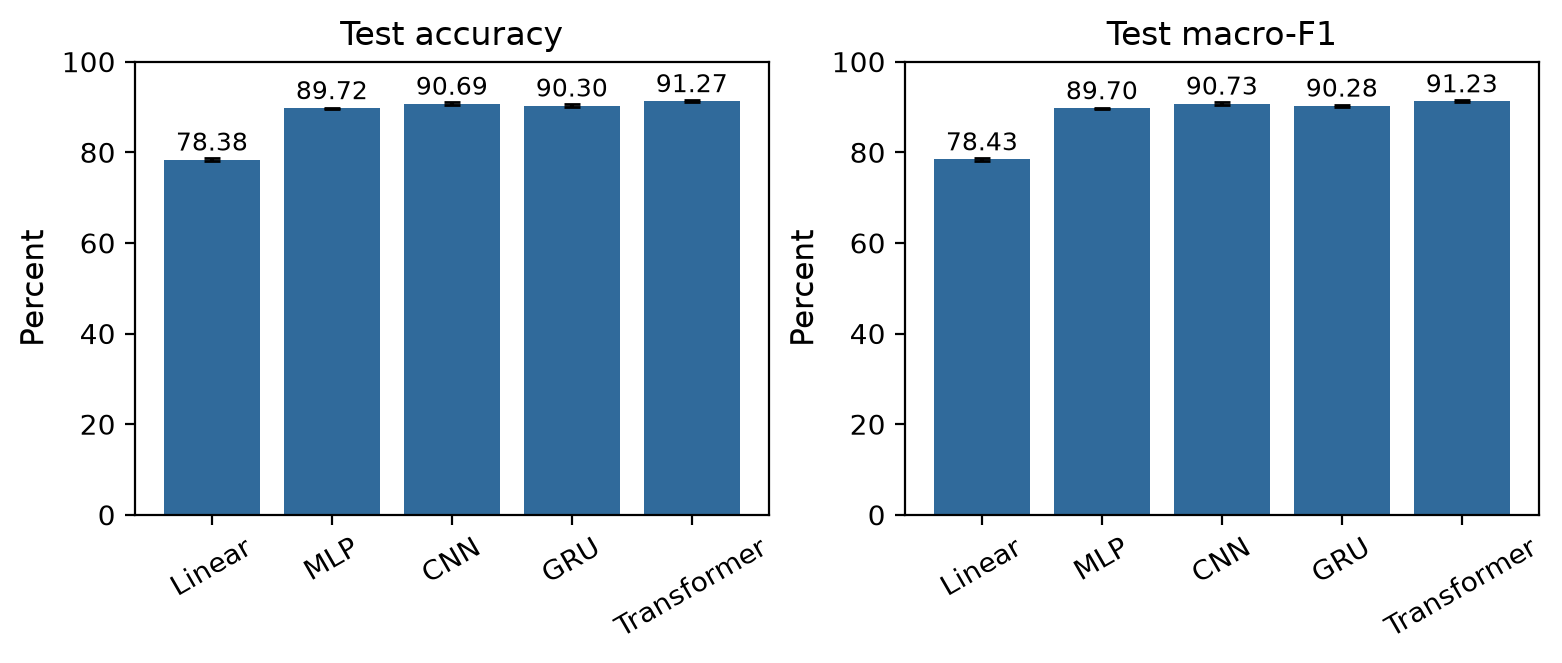
\includegraphics[width=\linewidth]{figures/comparison.png}
\caption{Official-test accuracy and macro-F1: mean with sample-SD error bars,
\(n=3\). Both axes retain the 0--100 percent scale.}
\label{fig:comparison}
\end{figure}

Table~\ref{tab:parameters} separates total, trainable and frozen parameter elements.
All five recorded architectures are fully trainable. Buffers are not parameters.
CNN uses about 72.9\% fewer parameters than Transformer while remaining close
in predictive quality; the larger MLP does not obtain the strongest scores.
\begin{table}[H]\centering\small
\caption{Exact parameter counts of the reported configurations.}
\label{tab:parameters}
\begin{tabular}{lrrr}
\toprule
Model & Total & Trainable & Frozen \\
\midrule
Linear & 7,850 & 7,850 & 0 \\
MLP & 235,146 & 235,146 & 0 \\
CNN & 28,426 & 28,426 & 0 \\
GRU & 61,962 & 61,962 & 0 \\
Transformer & 104,970 & 104,970 & 0 \\
\bottomrule
\end{tabular}

\end{table}
\FloatBarrier

\subsection{Learning Dynamics and Convergence}
Figures~\ref{fig:learn-linear}--\ref{fig:learn-transformer} show seed 67 for each
model. The vertical line marks the saved best-validation checkpoint, using
1-based epochs. The selected epoch need not be the final epoch.

\begin{figure}[H]\centering
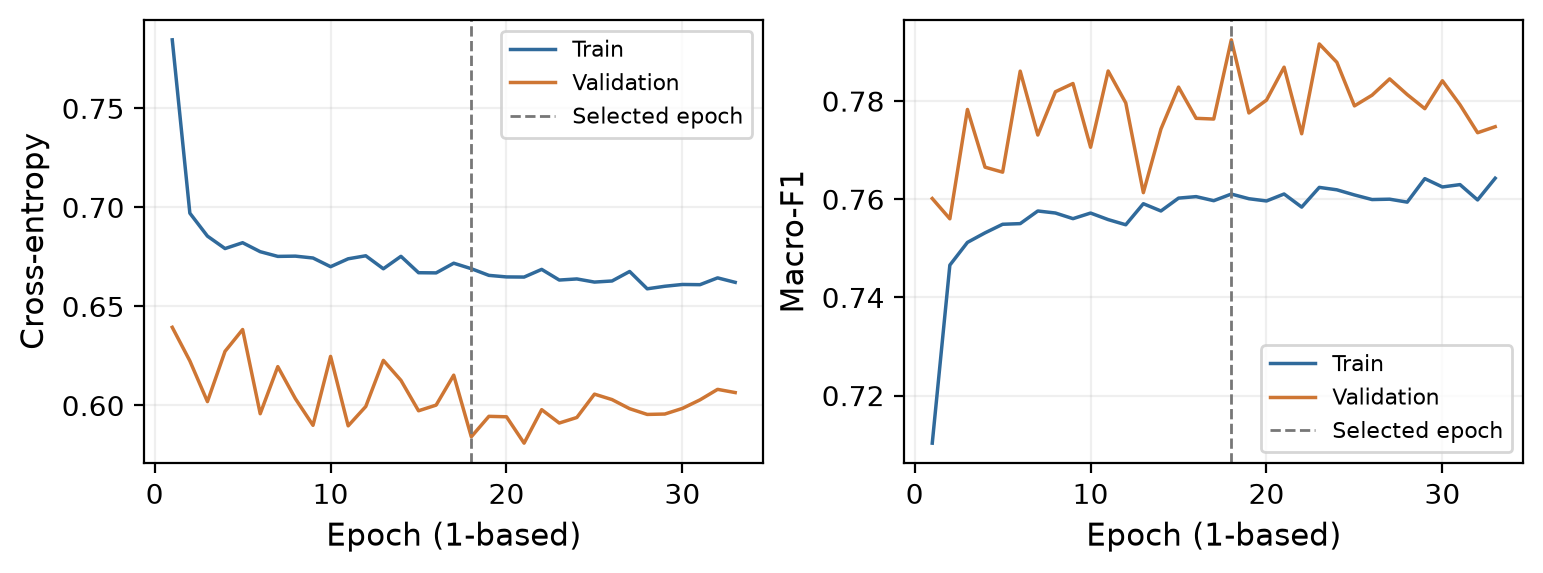
\includegraphics[width=\linewidth]{figures/learning_linear.png}
\caption{Linear learning history, seed 67: training/validation loss and macro-F1.}
\label{fig:learn-linear}
\end{figure}

\begin{figure}[H]\centering
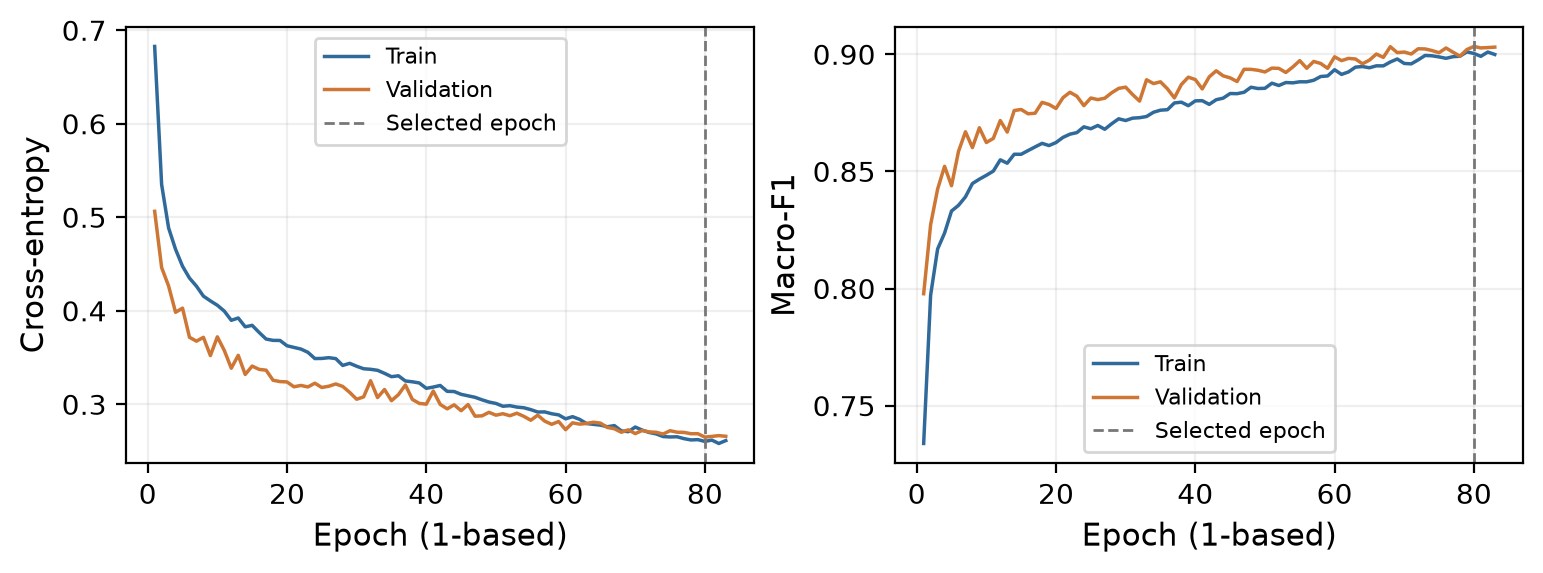
\includegraphics[width=\linewidth]{figures/learning_mlp.png}
\caption{MLP learning history, seed 67: training/validation loss and macro-F1.}
\label{fig:learn-mlp}
\end{figure}

\begin{figure}[H]\centering
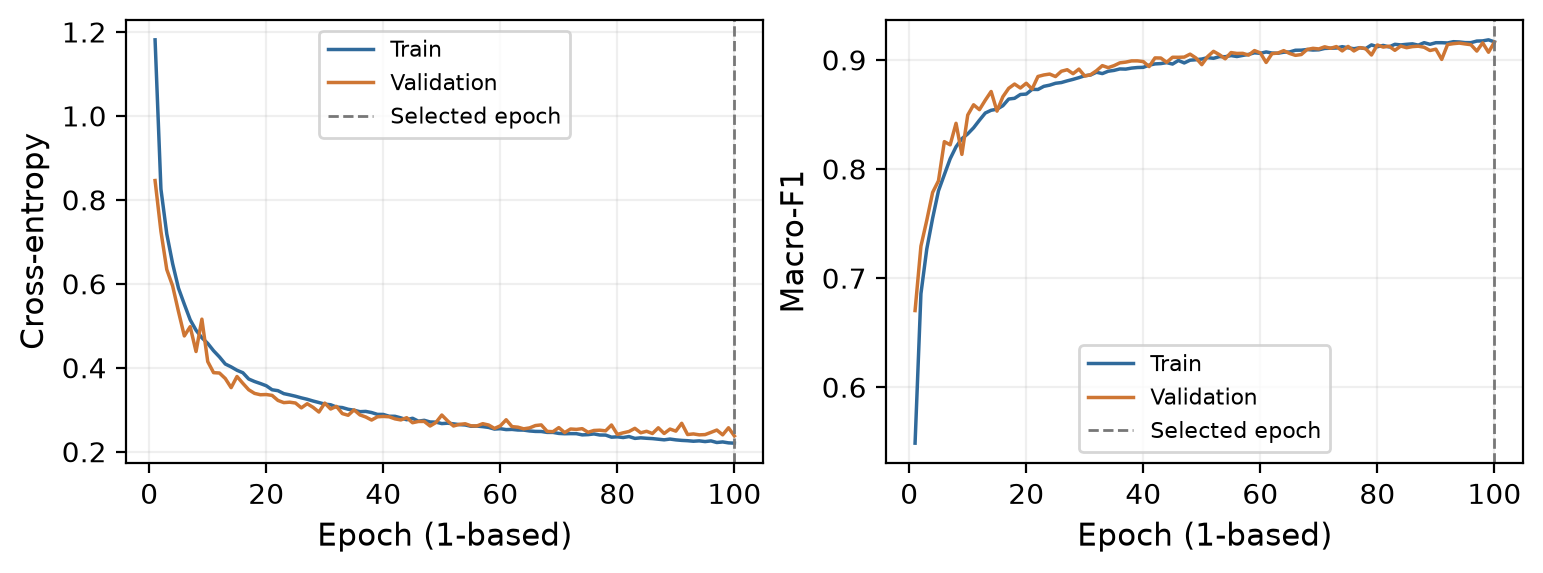
\includegraphics[width=\linewidth]{figures/learning_cnn.png}
\caption{CNN learning history, seed 67: training/validation loss and macro-F1.}
\label{fig:learn-cnn}
\end{figure}

\begin{figure}[H]\centering
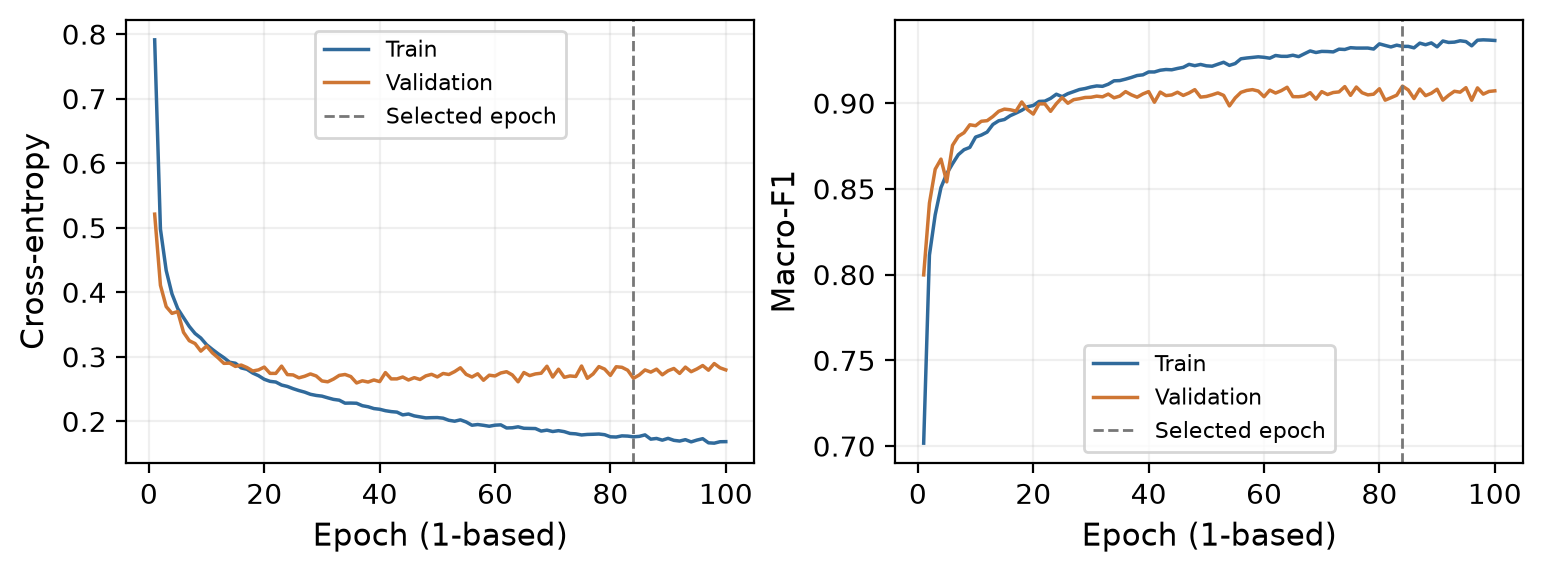
\includegraphics[width=\linewidth]{figures/learning_rnn.png}
\caption{GRU learning history, seed 67: training/validation loss and macro-F1.}
\label{fig:learn-rnn}
\end{figure}

\begin{figure}[H]\centering
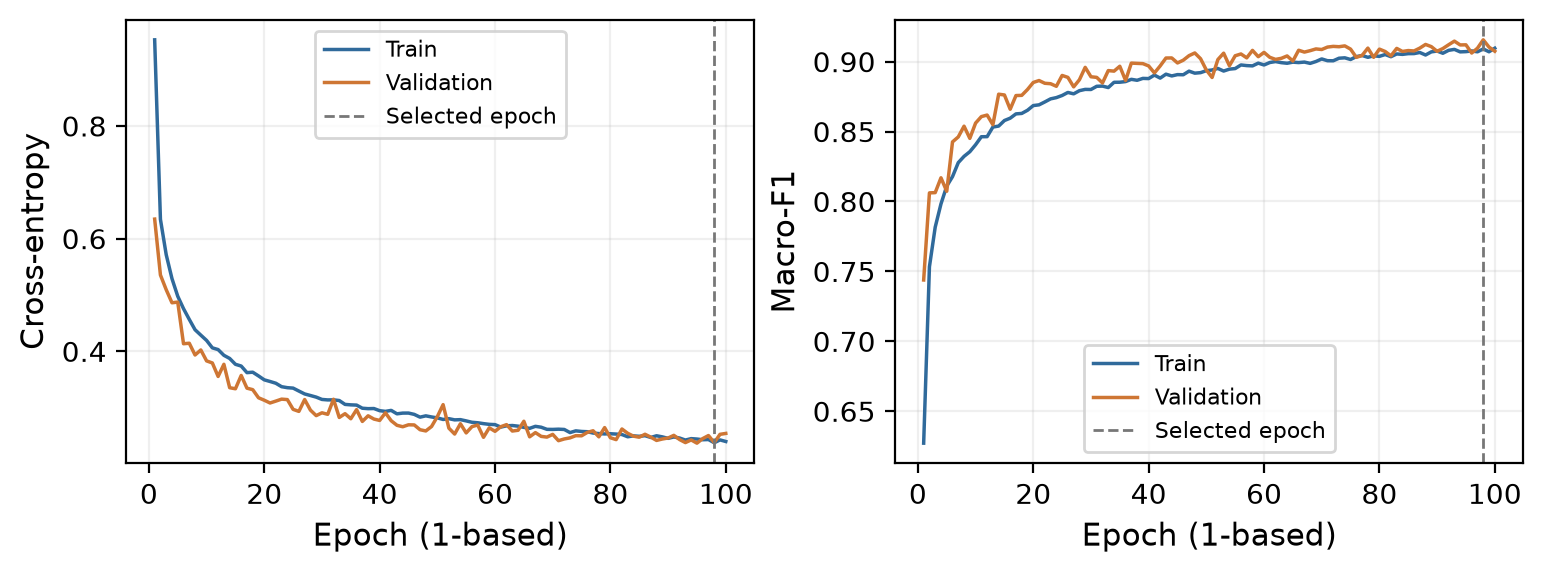
\includegraphics[width=\linewidth]{figures/learning_transformer.png}
\caption{Transformer learning history, seed 67: training/validation loss and macro-F1.}
\label{fig:learn-transformer}
\end{figure}

Linear stabilizes at much lower F1 and fluctuates after early improvement.
MLP, CNN and Transformer improve rapidly before making smaller late gains;
their observed training and validation curves remain relatively close.
These training curves include augmentation and dropout effects, while validation
uses deterministic preprocessing and evaluation mode.

GRU shows the clearest late divergence: training F1 continues improving while
validation F1 largely plateaus and validation loss rises slightly. Its seed-67
selected epoch is 84, before the final epoch 100. This pattern suggests that
continuing optimization does not keep improving held-out validation performance.
It does not prove a single causal mechanism. Best epochs for the other seed-67
runs are Linear 18, MLP 80, CNN 100 and Transformer 98.
\FloatBarrier

\subsection{Efficiency and Accuracy--Compute Trade-offs}
Table~\ref{tab:train-time} sums the saved \texttt{epoch\_seconds} values, each
of which surrounds training plus validation. It excludes full startup,
preparation and checkpoint overhead, and should not be read as isolated
forward/backward time.
\begin{table}[H]\centering\small
\caption{T4 train-and-validation epoch-loop cost. Epoch sequences and best
epochs are ordered by seeds 69420/67/69; times are mean \(\pm\) sample SD.}
\label{tab:train-time}
\begin{tabular}{lcr c}
\toprule
Model & Epochs & Loop time (min) & Best epochs \\
\midrule
Linear & 38 / 33 / 31 & 10.27 $\pm$ 1.05 & 30 / 18 / 16 \\
MLP & 100 / 83 / 100 & 29.85 $\pm$ 3.18 & 92 / 80 / 93 \\
CNN & 100 / 100 / 100 & 33.49 $\pm$ 0.44 & 100 / 100 / 81 \\
GRU & 100 / 100 / 100 & 32.89 $\pm$ 0.24 & 62 / 84 / 53 \\
Transformer & 100 / 100 / 100 & 38.39 $\pm$ 0.91 & 96 / 98 / 100 \\
\bottomrule
\end{tabular}

\end{table}
The Transformer has the largest observed loop cost (38.39 minutes), compared
with CNN's 33.49 minutes, a difference of about 4.90 minutes. Both use 100
epochs, but their per-epoch computation differs. Linear/MLP totals also reflect
their early-stopping policy and, for MLP, a shorter 83-epoch run. The MLP's
timing SD therefore includes a budget difference; it is not solely machine noise
or variation in model quality.

Table~\ref{tab:inference} reports the separate Windows CPU measurements under
Section~\ref{sec:environment}'s batch-64 forward-only protocol. A row averages
three per-checkpoint medians of 100 timed batches; SD describes those three
run-level values.
\begin{table}[H]\centering\small
\caption{Windows CPU forward-only timing: two threads, float32, batch 64,
20 warm-ups and 100 timed batches per checkpoint; \(n=3\).}
\label{tab:inference}
\begin{tabular}{lrrr}
\toprule
Model & Batch time (ms) & ms/image & Images/s \\
\midrule
Linear & 0.097 $\pm$ 0.003 & 0.001523 $\pm$ 0.000051 & 657237 $\pm$ 22106 \\
MLP & 1.151 $\pm$ 0.129 & 0.017987 $\pm$ 0.002016 & 56047 $\pm$ 6034 \\
CNN & 25.875 $\pm$ 2.663 & 0.404296 $\pm$ 0.041606 & 2491 $\pm$ 260 \\
GRU & 6.897 $\pm$ 2.059 & 0.107765 $\pm$ 0.032176 & 9776 $\pm$ 2494 \\
Transformer & 28.463 $\pm$ 3.584 & 0.444738 $\pm$ 0.056000 & 2273 $\pm$ 288 \\
\bottomrule
\end{tabular}

\end{table}
The Linear and MLP have much lower measured CPU cost than the other models.
CNN averages 0.404296 ms/image versus Transformer's 0.444738, so the Transformer
is about 10.0\% slower by these observed means. Their timing SDs are substantial,
and no formal claim of a stable speed ordering is made. GRU's mean is 0.107765
ms/image, giving a different quality--speed trade-off from its T4 training cost.
Throughput averages per-run rates; it need not equal the reciprocal of the rounded
aggregate latency.

These figures describe the documented CPU/library profile and preallocated input,
not end-to-end service performance. Parameter count alone does not predict runtime:
kernel structure, sequence processing and implementation matter, but their
individual contributions were not isolated. Deployment choices require measurements
on the intended hardware, batch size and input path.
\FloatBarrier

\subsection{Confusion Matrices and Class-Level Results}
\label{sec:confusion}
The following figures use the seed-67 official-test predictions; class metrics
quoted in the accompanying text refer to those same predictions.
They are representative single-run evidence; Table~\ref{tab:performance} remains
the three-seed comparison, and Appendix~\ref{app:class} reports aggregate class
metrics. Every figure uses the same raw-count color range, 0--1,000, and the same
class order.

There are 1,000 test examples per class. Consequently,
\(\mathrm{Recall}_c=C_{cc}/1000\); raw diagonal counts themselves are not recalls.
Because supports are equal, overall accuracy equals mean class recall.
Quoted precision, recall and F1 use the 0--1 scale. Full seed-level class metrics
are retained in the source CSV, and aggregate class tables appear in the appendix.

\clearpage
\subsubsection{Linear}
\begin{figure}[H]\centering
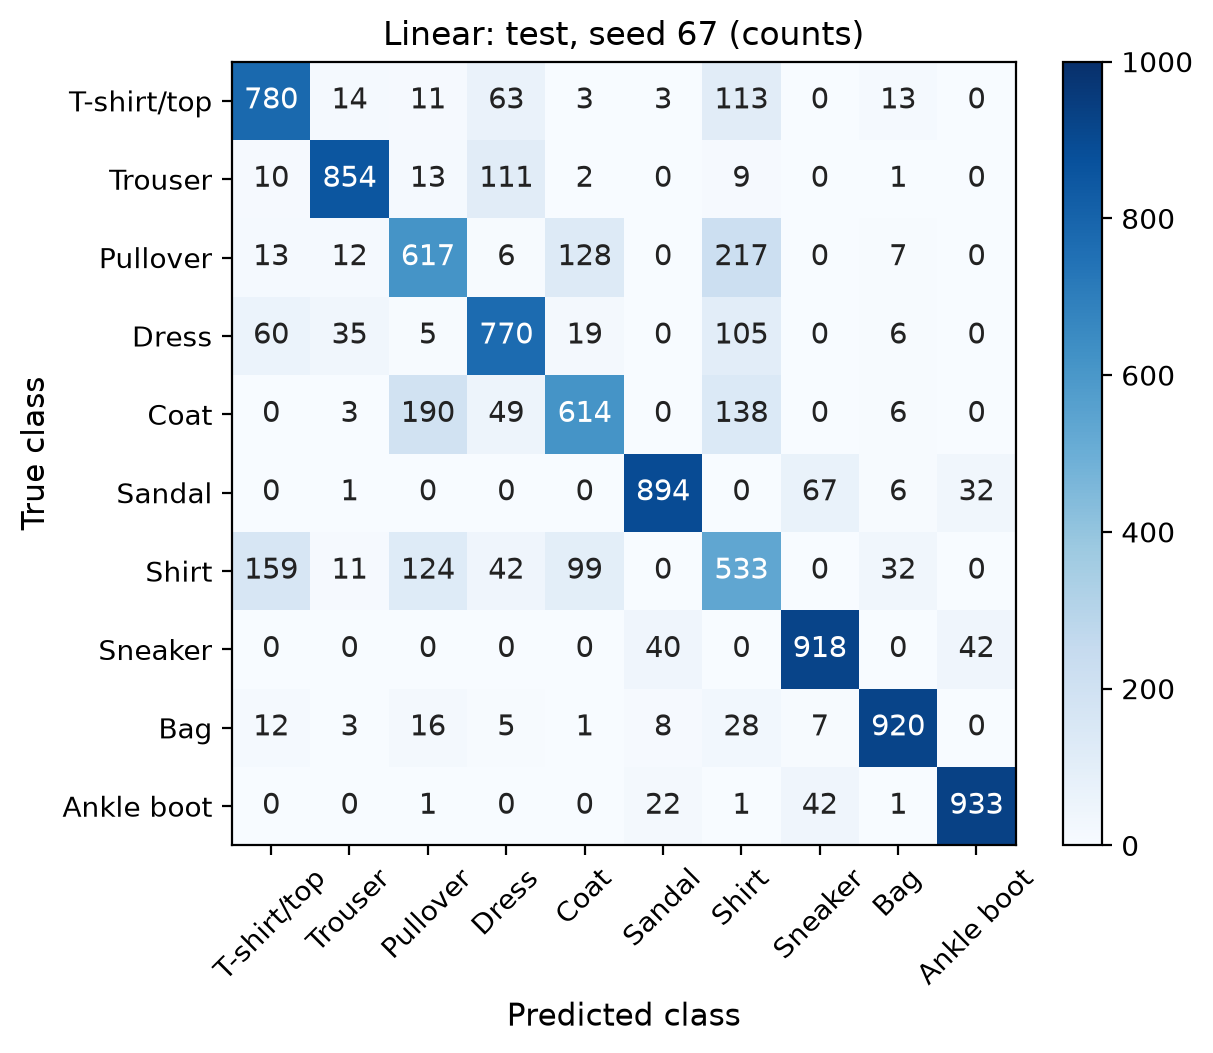
\includegraphics[width=.90\linewidth]{figures/confusion_linear.png}
\caption{Linear test confusion counts, seed 67; shared color scale 0--1,000.}
\label{fig:cm-linear}
\end{figure}
Linear's weakest class is Shirt (F1 0.497), with 159 Shirts predicted as
T-shirt/top, 124 as Pullover and 99 as Coat. Pullover/Coat confusion is also large:
128 Pullovers are predicted as Coat and 190 Coats as Pullover. This motivates
using nonlinear and spatial feature models, but the comparison does not isolate
representation from all other configuration differences.

\clearpage
\subsubsection{MLP}
\begin{figure}[H]\centering
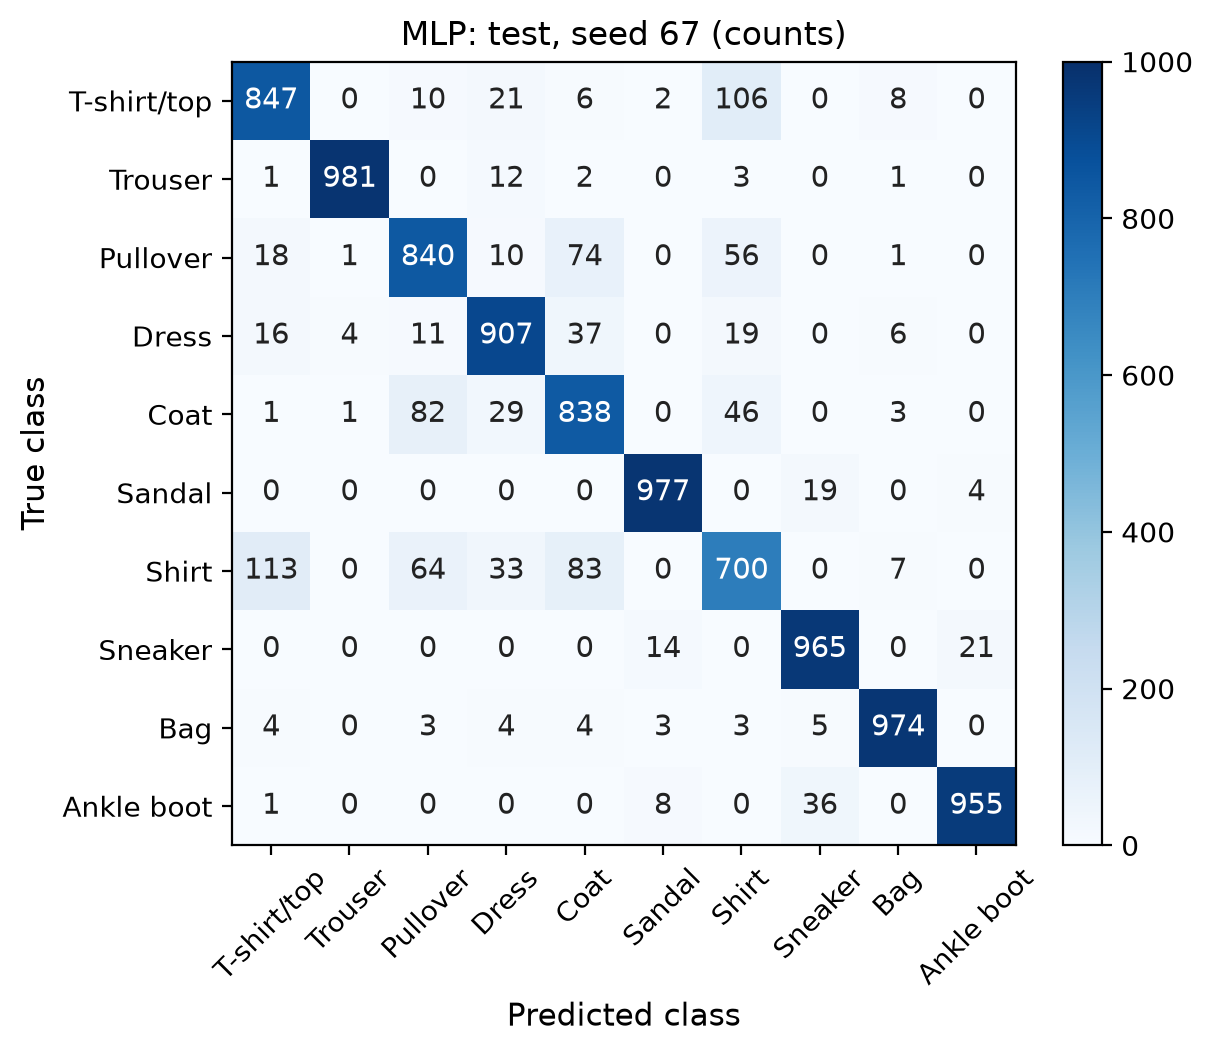
\includegraphics[width=.90\linewidth]{figures/confusion_mlp.png}
\caption{MLP test confusion counts, seed 67; shared color scale 0--1,000.}
\label{fig:cm-mlp}
\end{figure}
MLP improves overall accuracy to 89.84\% in this run. Trouser has F1 0.987,
while Shirt remains lowest at 0.724. There are 113 Shirt-to-T-shirt/top errors
and 106 in the reverse direction. Pullover--Coat errors persist (74 and 82 in
the two directions), showing that greater dense capacity does not eliminate
apparel ambiguity.

\clearpage
\subsubsection{CNN}
\begin{figure}[H]\centering
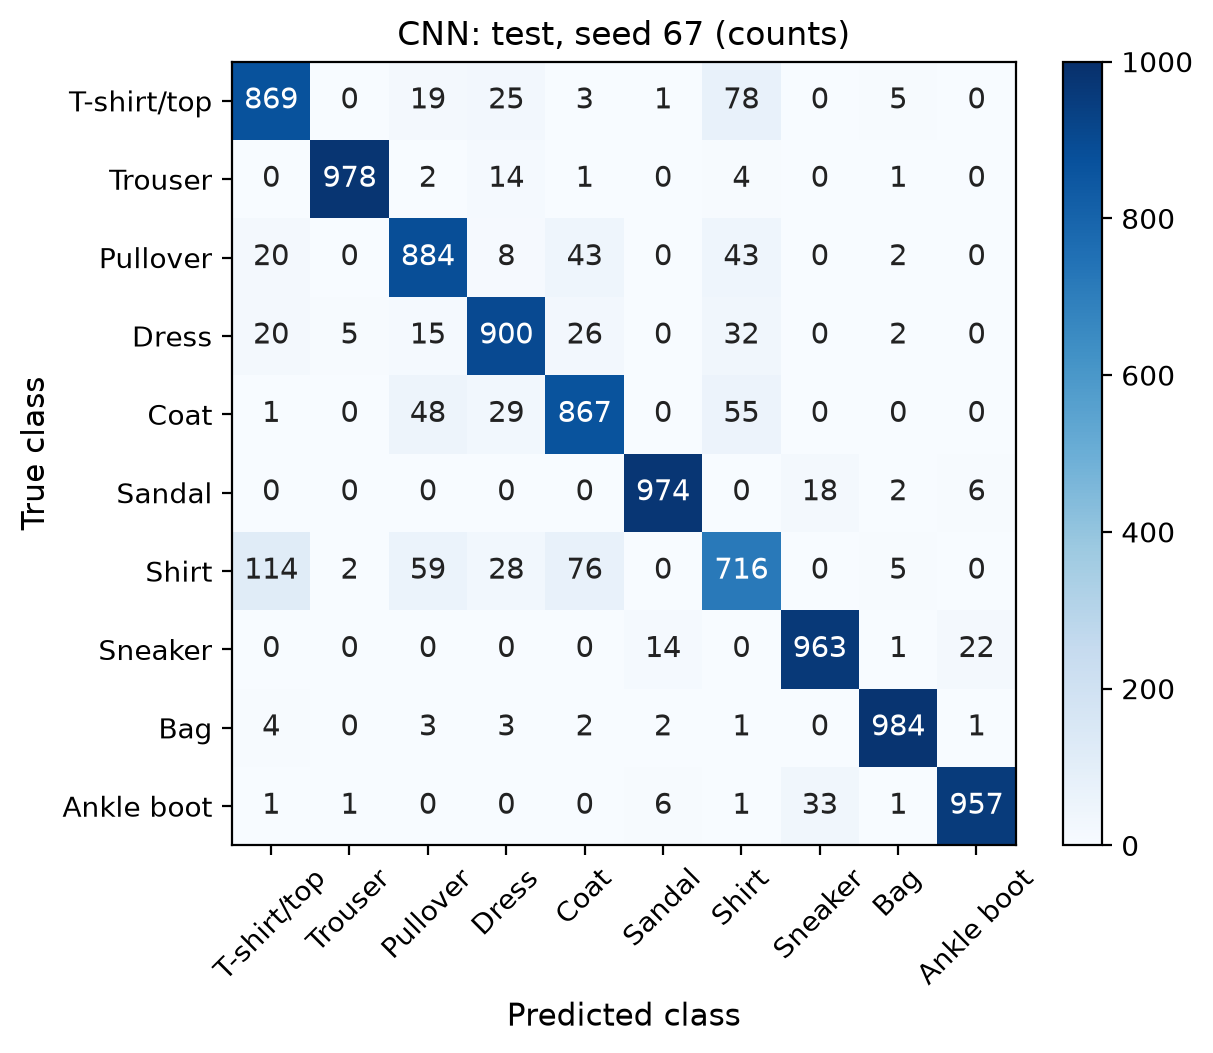
\includegraphics[width=.90\linewidth]{figures/confusion_cnn.png}
\caption{CNN test confusion counts, seed 67; shared color scale 0--1,000.}
\label{fig:cm-cnn}
\end{figure}
CNN reaches 90.92\% accuracy in this seed. Shirt remains weakest (F1 0.742);
114 Shirts are predicted as T-shirt/top, 76 as Coat and 59 as Pullover.
Pullover--Coat errors are lower than MLP's in both directions (43 and 48).
This is compatible with useful local image features, but is not a controlled
causal test of locality.

\clearpage
\subsubsection{GRU}
\begin{figure}[H]\centering
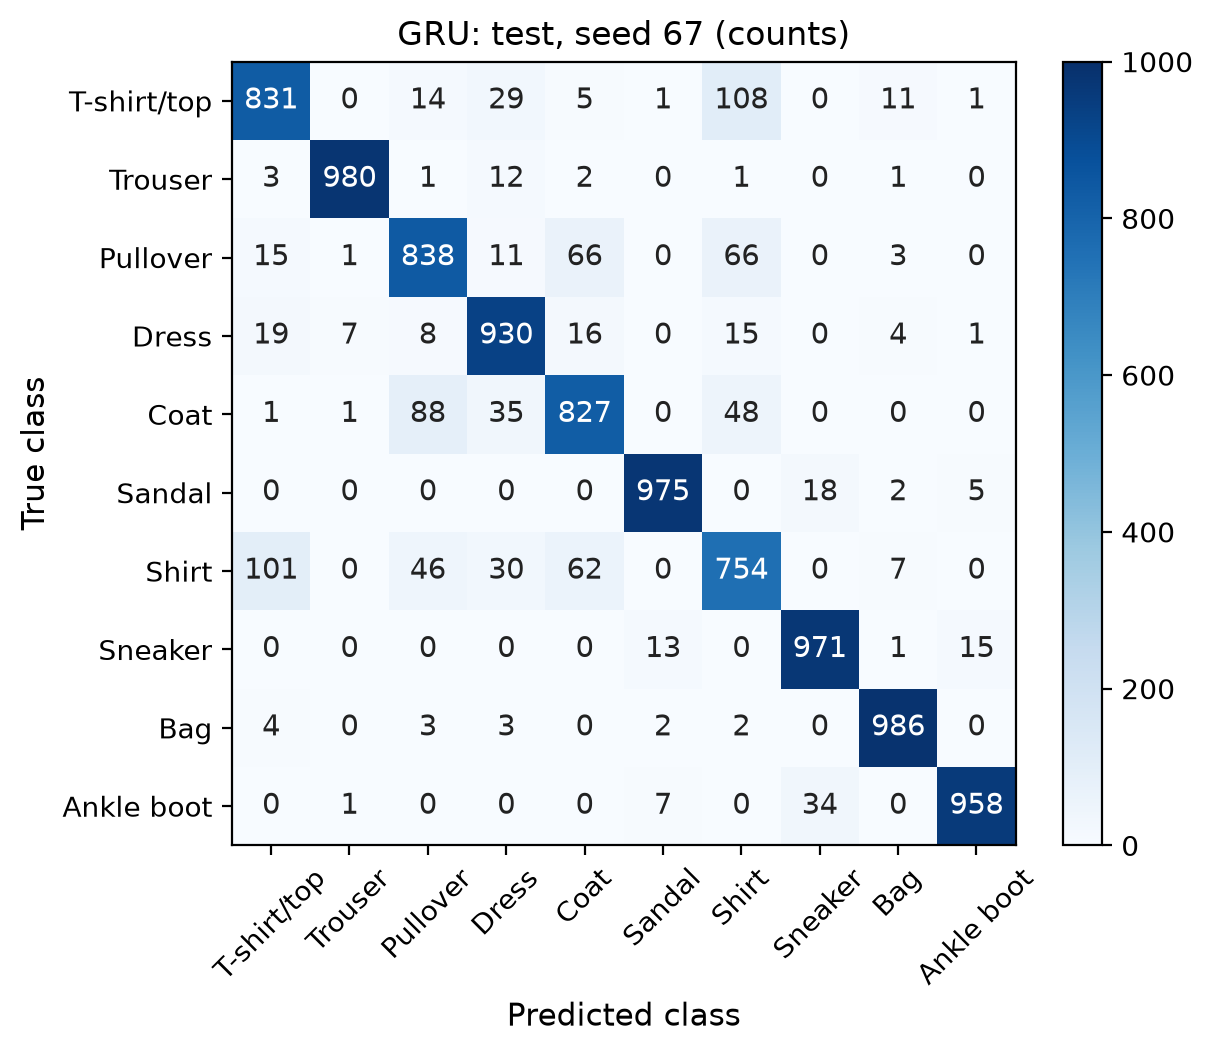
\includegraphics[width=.90\linewidth]{figures/confusion_rnn.png}
\caption{GRU test confusion counts, seed 67; shared color scale 0--1,000.}
\label{fig:cm-rnn}
\end{figure}
GRU reaches 90.50\% accuracy. Bag has its highest recall, 0.986; Dress
recall is 0.930. GRU has the highest Shirt recall among these five seed-67
models (0.754), although Shirt is still its lowest-F1 class (0.756).
Its overall score therefore does not reveal every class-level advantage.

\clearpage
\subsubsection{Transformer}
\begin{figure}[H]\centering
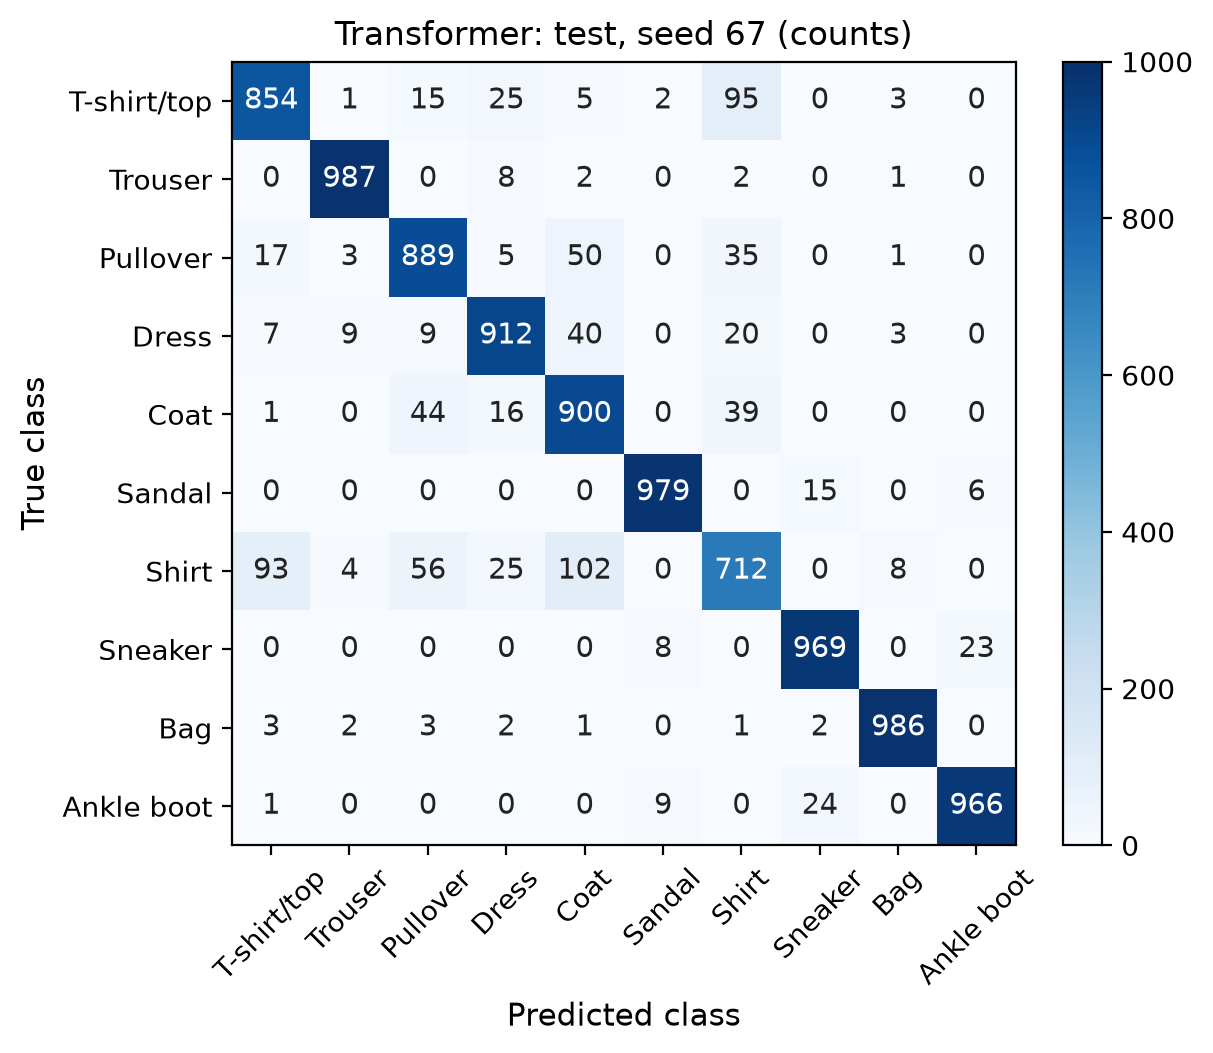
\includegraphics[width=.90\linewidth]{figures/confusion_transformer.png}
\caption{Transformer test confusion counts, seed 67; shared color scale 0--1,000.}
\label{fig:cm-transformer}
\end{figure}
Transformer reaches 91.54\% accuracy in seed 67 and has strong Bag
and Trouser F1 (0.985 and 0.984). Shirt remains weakest (F1 0.748), with 102
Shirts predicted as Coat, 93 as T-shirt/top and 56 as Pullover. Shirt precision
is higher than GRU's while recall is lower (0.712), illustrating a class-level
trade-off despite the strongest aggregate score.

\clearpage
\subsection{Qualitative Predictions and Error Analysis}
\label{sec:qualitative}
Each gallery below contains three correct, three difficult-correct and three
confidently incorrect examples from the same seed-67 test run. Correct examples
use the common IDs 0, 1 and 10 for all models; difficult-correct examples are
the three lowest-confidence correct predictions per model, and errors are the
three highest-confidence mistakes. Other IDs therefore vary across models.
The IDs identify official-test images; probabilities are rounded to three decimals.
These selected galleries illustrate behavior, not the prevalence of an error type.


\begin{figure}[H]\centering
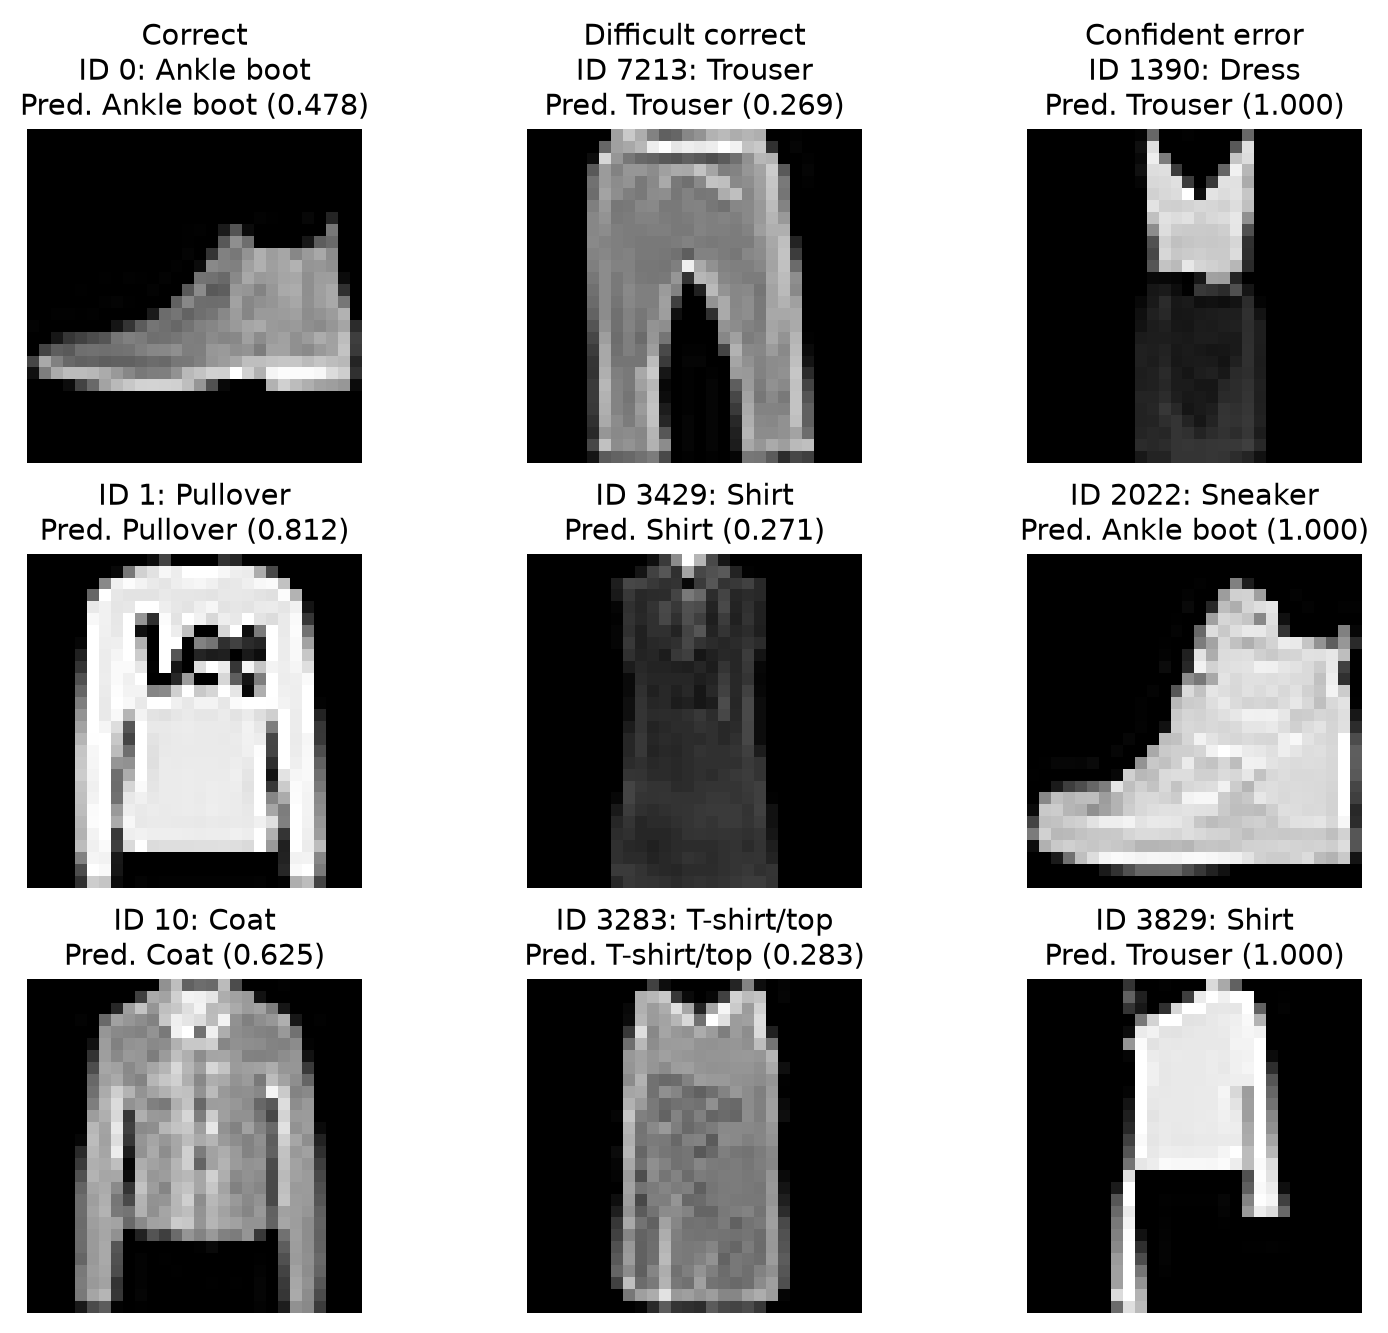
\includegraphics[width=.84\linewidth]{figures/gallery_linear.png}
\caption{Linear: common correct examples (left), low-confidence correct cases
(middle) and high-confidence errors (right), test seed 67.}
\label{fig:gallery-linear}
\end{figure}

\clearpage
\begin{figure}[H]\centering
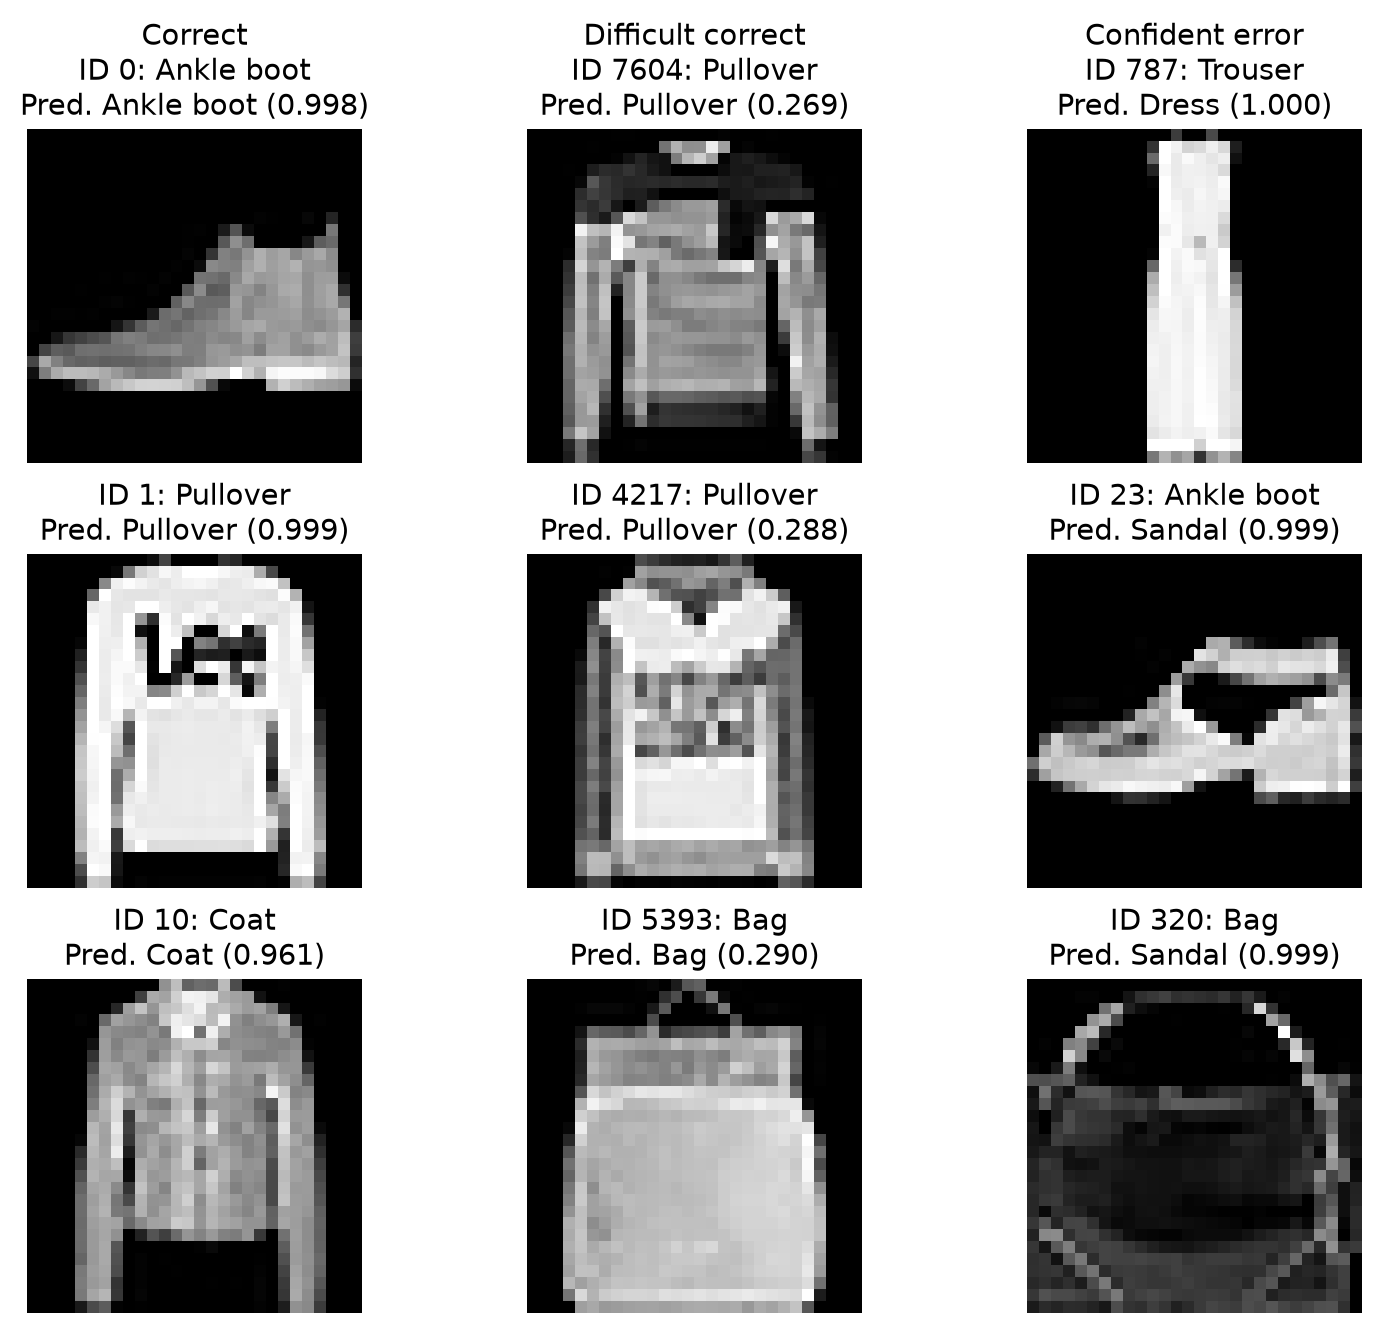
\includegraphics[width=.96\linewidth]{figures/gallery_mlp.png}
\caption{MLP: common correct examples (left), low-confidence correct cases
(middle) and high-confidence errors (right), test seed 67.}
\label{fig:gallery-mlp}
\end{figure}

\clearpage
\begin{figure}[H]\centering
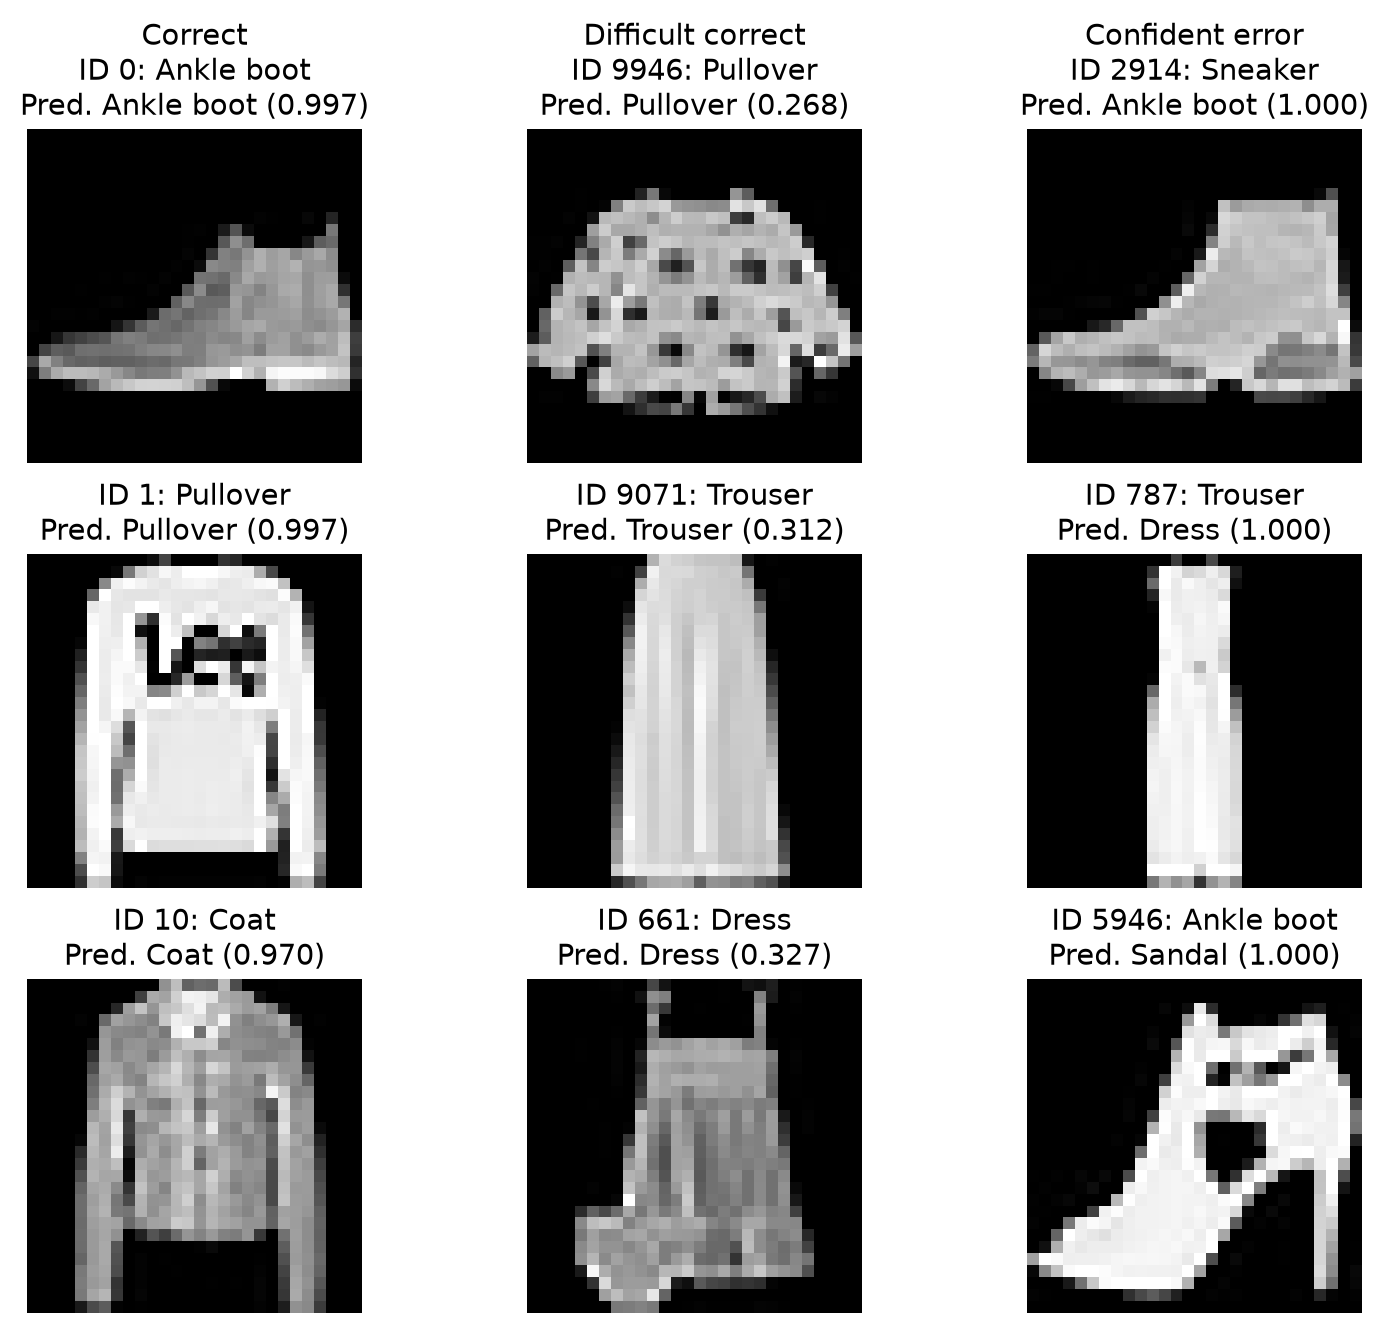
\includegraphics[width=.96\linewidth]{figures/gallery_cnn.png}
\caption{CNN: common correct examples (left), low-confidence correct cases
(middle) and high-confidence errors (right), test seed 67.}
\label{fig:gallery-cnn}
\end{figure}

\clearpage
\begin{figure}[H]\centering
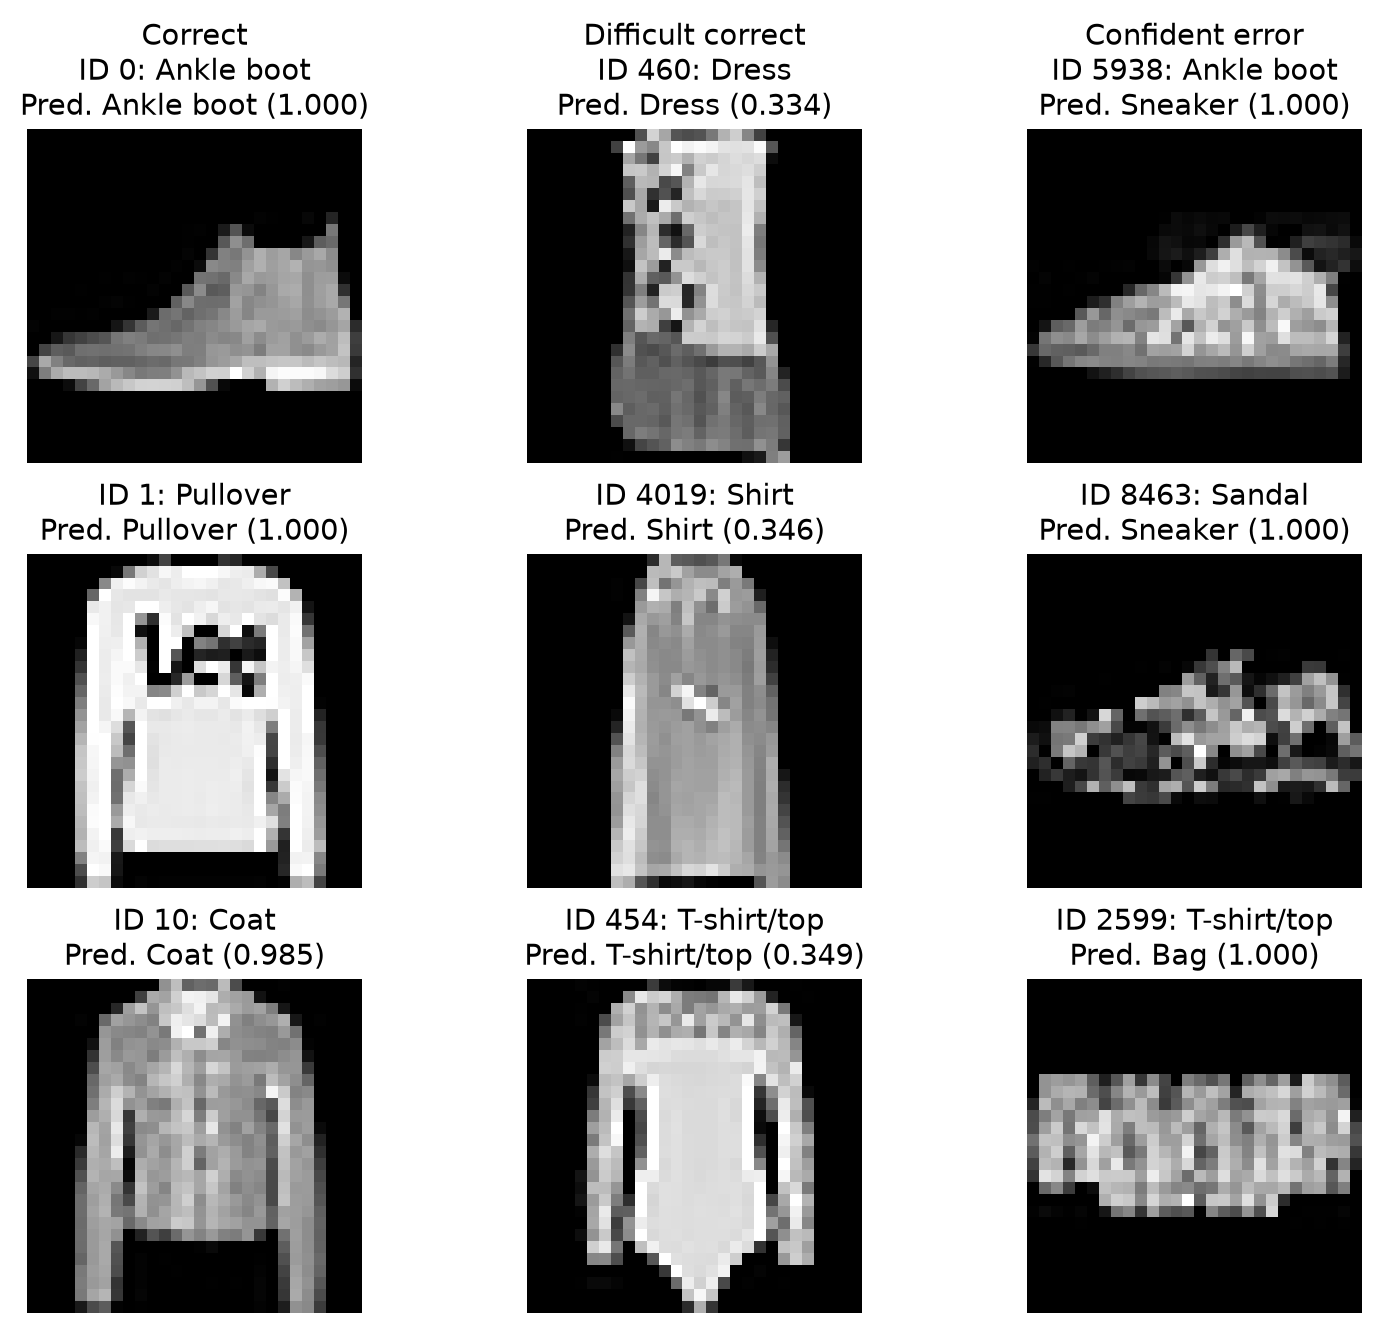
\includegraphics[width=.96\linewidth]{figures/gallery_rnn.png}
\caption{GRU: common correct examples (left), low-confidence correct cases
(middle) and high-confidence errors (right), test seed 67.}
\label{fig:gallery-rnn}
\end{figure}

\clearpage
\begin{figure}[H]\centering
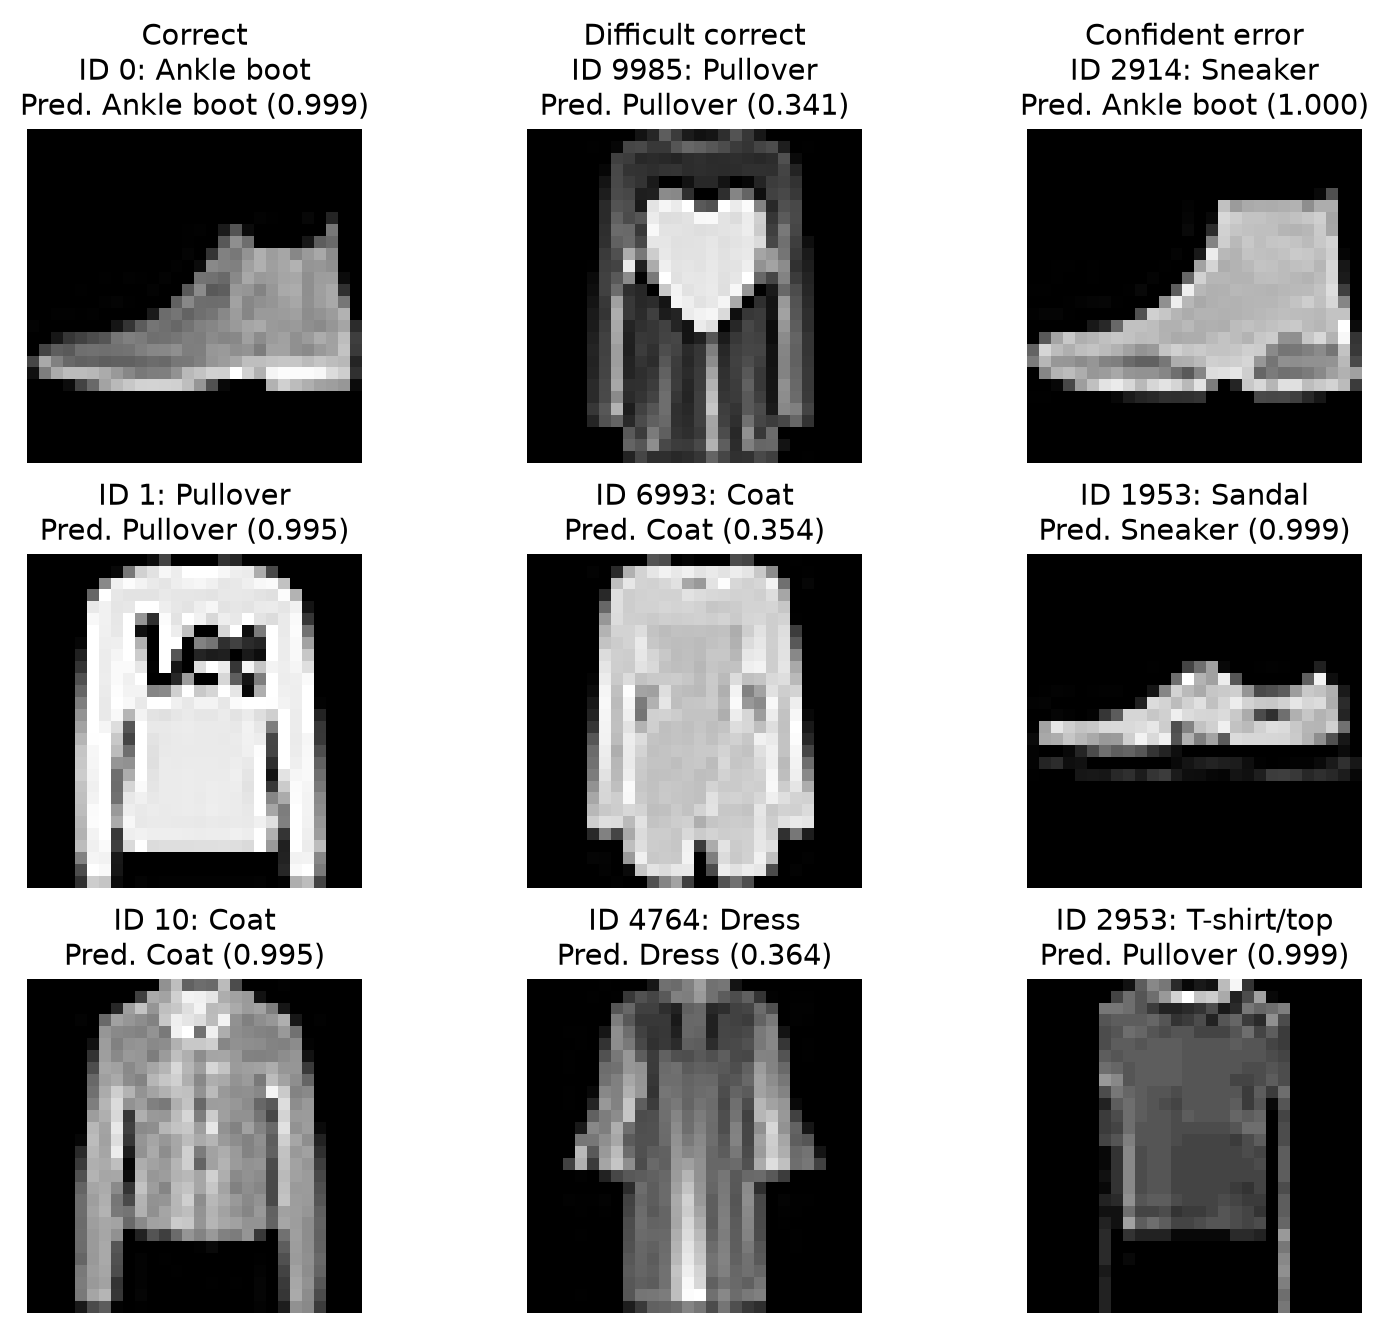
\includegraphics[width=.96\linewidth]{figures/gallery_transformer.png}
\caption{Transformer: common correct examples (left), low-confidence correct cases
(middle) and high-confidence errors (right), test seed 67.}
\label{fig:gallery-transformer}
\end{figure}

\FloatBarrier
The common example ID 0 (Ankle boot) is correct with confidence approximately
0.478 for Linear and near 1.0 for the nonlinear models. Conversely, both MLP
and CNN confidently predict Dress for true Trouser ID 787. Thus, a high softmax
score does not guarantee correctness. Low-confidence correct cases also show
that uncertainty and the final argmax label are distinct.

The class matrices quantify recurrent upper-body confusions; footwear galleries
show additional Sandal/Sneaker/Ankle-boot ambiguity. Plausible explanations are
shared silhouettes, limited resolution and missing texture cues, but the
present artifacts do not prove label errors or identify a unique cause.
Several focused follow-ups would address these patterns:
\begin{itemize}
\item Apparel confusions: inspect validated examples of Shirt/T-shirt/top/Coat/
Pullover and compare representations under matched training/parameter budgets.
This would test whether local or sequence features explain the observed gap.
\item Footwear confusions: measure pair-specific error rates and test a controlled
augmentation change while keeping model initialization and evaluation fixed.
The present galleries alone cannot establish whether augmentation would help.
\item Confident mistakes: assess reliability or calibration error on validation,
then evaluate a validation-fitted procedure under a fresh or preregistered
held-out protocol. A gallery is insufficient to claim population calibration.
\end{itemize}
These are proposed investigations, not completed ablations or promised gains.

\subsection{Representation and Inductive-Bias Discussion}
Linear assigns each class one global weighted pixel combination, with no hidden
feature hierarchy. Its low scores and severe apparel confusions are consistent
with limited expressiveness. Adding nonlinear dense layers improves test accuracy
by about 11.34 percentage points, but MLP remains below CNN and Transformer
despite having the largest parameter count.

The CNN's local connectivity and shared filters suit spatial image patterns.
It achieves close-to-leading quality with only 28,426 parameters. GRU instead
aggregates an ordered row sequence; its high seed-67 Shirt recall shows that
some class-level strengths are not captured by the overall ranking. No row/
column comparison was run, so the contribution of traversal order is unisolated.

The Transformer can combine information from distant patches through attention,
using learned position parameters to distinguish their locations. Its best
aggregate quality does not remove the shared Shirt/Coat ambiguity.
The results support these configurations as practical alternatives, but do not
prove that attention, locality or recurrence alone caused the measured differences.

\subsection{Limitations}
The evidence covers Fashion-MNIST, one effective configuration per family,
three seeds and one shared split. There is no matched-budget ablation, external
dataset, robustness benchmark or significance test. The repeated evaluations
reuse the same images, and selecting checkpoints on validation makes validation
scores optimistic for final comparison.

Epoch-loop cost combines training/validation and differs in completed epochs.
Training, classification evaluation and inference timing use distinct environments.
The Windows timing profile uses preallocated zeros and excludes I/O/transfer;
its amortized batch-64 cost does not predict batch-one or real-service latency.
Python patch-version variation, library differences and unrecorded friendly CPU
model name further limit exact cross-machine reproduction. The raw Windows timing
samples are retained; no unverified Colab timing table is substituted for them.

Example selection is deterministic but selective; images are not an uncertainty
or calibration sample. No perceptual-duplicate removal or independent label audit
was performed. The proposed explanations and follow-ups remain hypotheses.

\subsection{Conclusion}
The four research questions can be answered within these limits:
\begin{enumerate}
\item \textbf{Predictive quality.} Transformer leads at 91.267\% test accuracy
and 91.234\% macro-F1; CNN follows at 90.690\% and 90.726\%.
\item \textbf{Representation and errors.} Spatial and patch-token configurations
perform strongly, but similar apparel remains difficult. Architecture alone
was not isolated as the cause.
\item \textbf{Efficiency.} CNN has 72.9\% fewer parameters and 4.90 fewer
minutes of T4 epoch-loop time than Transformer. Their Windows CPU times are
0.404/0.445 ms per image; the preferred trade-off depends on the device.
\item \textbf{Seed consistency.} Test-accuracy SD is at most 0.324 percentage
points. All three paired Transformer--CNN differences are positive, without
establishing statistical significance.
\end{enumerate}
The measured outcome is a configuration-specific trade-off on Fashion-MNIST,
not a general ordering of architecture families for image classification.
\FloatBarrier

\clearpage
\section*{Reproducibility and Artifact Access}
\addcontentsline{toc}{section}{Reproducibility and Artifact Access}
The report follows the handbook's three-part structure and distinguishes measured
results from proposed follow-ups.\citep{handbook}
The source repository is
\href{https://github.com/TuanKhai1210/Deep-Learning-Benchmark-Suite}{Deep-Learning-Benchmark-Suite};
the assignment entry point is
\href{https://tuankhai1210.github.io/Deep-Learning-Benchmark-Suite/a1.html}{the A1 project page}.
The reported run revision is:
\begin{center}\small\texttt{a8539bee778d99e2902a1dd36aa157c6ebb3a42c}\end{center}
The run artifacts and snapshots, rather than an older README status paragraph,
define the effective configurations. Appendix~\ref{app:runs} maps all 15 results
to their run IDs; the source package includes exact effective JSON configs,
per-run metrics, raw timing samples and input/checkpoint hashes under
\texttt{evidence/}.

Original checkpoints are maintained in the group's Drive artifact bundle
\path{MyDrive/dlbench_a1_main/main/}, with one run directory per ID.
They are not embedded in the LaTeX archive and no anonymous public checkpoint
download URL is asserted. Readers without that bundle can reconstruct the
models by training the included effective configs at the pinned source revision.
This provides a reconstruction route rather than claiming current access
permissions to the group's Drive.

For a Linux/Colab CUDA environment, the following installation identifies the
main recorded tensor-library builds. Python patch versions and operational
differences remain as described in Section~\ref{sec:environment}.
\begin{lstlisting}[basicstyle=\ttfamily\footnotesize,breaklines=true,frame=single]
git clone https://github.com/TuanKhai1210/Deep-Learning-Benchmark-Suite.git
cd Deep-Learning-Benchmark-Suite
git checkout a8539bee778d99e2902a1dd36aa157c6ebb3a42c
python -m pip install torch==2.11.0 torchvision==0.26.0 --index-url https://download.pytorch.org/whl/cu130
python -m pip install numpy==2.1.3
python -m pip install -e ".[ml]"
\end{lstlisting}
Official previous-version installation instructions document these builds.\citep{pytorchversions}
The effective configs and the environment records govern reconstruction;
installing unpinned optional extras alone is not a complete environment lock.

The included \path{reproduction/reproduce.py} reads a selected saved config,
requires the pinned repository revision and changes only explicit operational
paths/device settings. Its default action prints the resolved configuration;
training requires the explicit action below. In this example the report
source archive has been extracted to \texttt{/content/A1\_Final}:
\begin{lstlisting}[basicstyle=\ttfamily\footnotesize,breaklines=true,frame=single]
python /content/A1_Final/reproduction/reproduce.py \
  --repo-root . --model cnn --seed 67 --action train \
  --data-root data --output-root runs/a1_reproduction --device cuda
\end{lstlisting}
Repeat with the five model names \texttt{linear, mlp, cnn, rnn, transformer}
and seeds 69420, 67, 69. A new run may differ numerically because exact cross-machine
or cross-version bitwise reproduction has not been established.
Evaluation of a trusted saved checkpoint requires an explicit action and path:
\begin{lstlisting}[basicstyle=\ttfamily\footnotesize,breaklines=true,frame=single]
python /content/A1_Final/reproduction/reproduce.py \
  --repo-root . --model cnn --seed 67 --action test \
  --checkpoint /content/drive/MyDrive/dlbench_a1_main/main/a1_cnn_main_seed67_20261023-030133_702c4e/best.pt \
  --data-root data --device cpu
\end{lstlisting}
The source package also retains the one-pass evaluation notebook and timing-only
notebook in \texttt{reproduction/}. Their outputs preserve split/device labels
and completion identities. Regenerating report tables and figures from existing
artifacts uses \path{tools/build_assets.py}; it performs no model training or
checkpoint inference.

\section*{Member Contributions and AI Usage Disclosure}
\addcontentsline{toc}{section}{Member Contributions and AI Usage Disclosure}
The task division follows the project's recorded ownership: Nguyen Hao Thien
is responsible for data/EDA/preprocessing and Linear/CNN; Nguyen Anh Khoa for
the shared training/evaluation engine, MLP/GRU and metrics/checkpointing;
Ta Tuan Khai for Transformer, configuration/artifacts, integration and report
reproducibility. Shared interfaces and results require cross-member review.
The cover sheet retains the group's supplied completion declarations; automated
artifact checks do not independently measure individual contribution percentages.

AI assistance was used and is disclosed below. Historical details come from
the repository's \texttt{AI\_USAGE.md}, copied into the source package as
\path{evidence/AI_USAGE_source.md}. Model/version labels in that log are
reported as recorded rather than independently certified service identifiers.
\begin{table}[H]\centering\small
\caption{Recorded AI tools, users and development scope.}
\label{tab:ai}
\begin{tabularx}{\linewidth}{>{\raggedright\arraybackslash}p{30mm}>{\raggedright\arraybackslash}p{29mm}>{\raggedright\arraybackslash}X}
\toprule Tool/model as recorded & Member & Stage and affected work\\\midrule
OpenAI Codex & Ta Tuan Khai & Aug.--Oct.\ 2026: protocol, artifacts, Transformer support,
analysis, source correction and report generation\\
Gemini & Nguyen Hao Thien; Nguyen Anh Khoa & Sep.\ 2026: data/EDA, metrics/checkpoints,
trainer tests and analysis notebook\\
GitHub Copilot & Nguyen Anh Khoa & Sep.\ 2026: MLP/trainer tests and optimizer support\\
OpenAI ChatGPT & Nguyen Anh Khoa & Sep.\ 2026: trainer test-generation support\\
\bottomrule
\end{tabularx}
\end{table}

The historical log names Codex 5.6 Sol and GPT-6 in selected entries, Gemini
3.8 Flash and 3.1 Pro (High), and ChatGPT 5.6 Luna. Other serving model IDs
were not recorded. Representative prompt summaries include explaining leakage-free EDA and stratified
splits (Thien), identifying states needed for training resumption and generating
metric/trainer tests (Khoa), and making artifacts traceable to configs/checkpoints
and completing the LaTeX report from verified runs (Khai).
Historical log entries record student checks against the handbook, source interfaces,
PyTorch documentation and tests. They do not establish that AI output is correct
without those checks.

For the 23--26 October report/analysis work, Khai used Codex; the exact serving
model identifier for every interaction was not retained. AI proposed and edited
report prose, generated aggregation/plotting helpers, corrected source/report
inconsistencies, and helped assemble the final document. The current automated
verification recomputes aggregates from saved predictions/metrics, checks source
and checkpoint identities, verifies raw dataset resources, and compiles/inspects
the PDF. Official documentation and papers support the theoretical descriptions.
The team remains responsible for the interpretation and final verification of
its submission; this disclosure does not assert an unrecorded human sign-off.
Additional session detail is retained in \path{evidence/AI_USAGE_report.md}.
\FloatBarrier

\clearpage
\begin{thebibliography}{9}
\bibitem{fashion}
H. Xiao, K. Rasul and R. Vollgraf.
\emph{Fashion-MNIST: a Novel Image Dataset for Benchmarking Machine Learning Algorithms}.
2017. \url{https://arxiv.org/abs/1708.07747}.
\bibitem{fashionlicense}
Zalando Research. \emph{Fashion-MNIST repository and MIT License}.
2017. \url{https://github.com/zalandoresearch/fashion-mnist/blob/master/LICENSE}.
Accessed 26 October 2026.
\bibitem{attention}
A. Vaswani et al. \emph{Attention Is All You Need}.
Advances in Neural Information Processing Systems, 2017.
\url{https://arxiv.org/abs/1706.03762}.
\bibitem{pytorchgru}
PyTorch contributors. \emph{torch.nn.GRU, PyTorch 2.11 documentation}.
\url{https://docs.pytorch.org/docs/2.11/generated/torch.nn.GRU.html}.
Accessed 26 October 2026.
\bibitem{pytorchce}
PyTorch contributors. \emph{CrossEntropyLoss, PyTorch 2.11 documentation}.
\url{https://docs.pytorch.org/docs/2.11/generated/torch.nn.CrossEntropyLoss.html}.
Accessed 26 October 2026.
\bibitem{pytorchversions}
PyTorch contributors. \emph{Installing previous versions of PyTorch}.
\url{https://pytorch.org/get-started/previous-versions/}. Accessed 26 October 2026.
\bibitem{project}
Tiki-taka. \emph{Deep Learning Benchmark Suite}, source revision a8539be.
\url{https://github.com/TuanKhai1210/Deep-Learning-Benchmark-Suite}.
\bibitem{handbook}
CO3133, Semester 261. \emph{Course Project Handbook}, revision 14 September 2026.
Course-provided document; Sections 3--5 and 8--14.
\end{thebibliography}

\clearpage
\appendix
\section{Full Configurations and Architecture Details}
\label{app:configs}
The source package contains all 15 effective config snapshots under
\path{evidence/configs/}. Within each model, seeds change but architecture,
data/evaluation settings and training policy remain fixed. The common protocol
uses Fashion-MNIST, split seed 36, batch 64, Adam at \(10^{-3}\), weight decay
0, a 100-epoch cap and validation macro-F1 checkpoint selection.

\begin{table}[H]\centering\small
\caption{Effective model/training settings; detailed snapshots are included in the source.}
\begin{tabularx}{\linewidth}{lYY}
\toprule Model & Architecture & Model-specific training/regularization\\\midrule
Linear & 784 to 10 & Cosine to \(10^{-5}\); patience 15, min-delta 0.001\\
MLP & 784--256--128--10; ReLU & Hidden dropout 0.1; same cosine/patience as Linear\\
CNN & Channels 32/64; 3-by-3 kernels; max pooling; 64--128--10 head & Head dropout 0.1; no scheduler/early stop\\
GRU & Rows; input 28; hidden 128; one layer, one direction & No inter-layer dropout; no scheduler/early stop\\
Transformer & Patch 4; width 64; four heads; two blocks; FFN width 256 & Dropout 0.1; no scheduler/early stop\\
\bottomrule
\end{tabularx}
\end{table}
The saved configs also identify operational paths and the source configuration
modules. Device/path overrides used for later CPU stages are recorded separately,
not silently presented as the original T4 training setup. Parameter elements are
counted once through the model's parameter iterator; buffers are excluded and
\texttt{requires\_grad} determines trainability.
\FloatBarrier

\section{Per-Seed Results and Run Provenance}
\label{app:runs}
Table~\ref{tab:seeds} reports all seeds. Accuracy/F1 are percentages and the
selected epoch is 1-based; the source history itself uses 0-based indices.
There is no best-test-seed selection.
\begin{table}[H]\centering\footnotesize
\caption{All 15 selected checkpoints and their evaluation results.}
\label{tab:seeds}
\begin{tabular}{lrrrrrrr}
\toprule
Model & Seed & Epochs & Best & Val. acc. & Test acc. & Test F1 & Test CE \\
\midrule
Linear & 69420 & 38 & 30 & 79.16 & 78.12 & 78.098 & 0.61253 \\
Linear & 67 & 33 & 18 & 79.17 & 78.33 & 78.478 & 0.60811 \\
Linear & 69 & 31 & 16 & 79.47 & 78.68 & 78.706 & 0.61362 \\
MLP & 69420 & 100 & 92 & 90.15 & 89.67 & 89.647 & 0.29002 \\
MLP & 67 & 83 & 80 & 90.38 & 89.84 & 89.806 & 0.28514 \\
MLP & 69 & 100 & 93 & 90.47 & 89.65 & 89.641 & 0.28903 \\
CNN & 69420 & 100 & 100 & 91.43 & 90.32 & 90.423 & 0.27405 \\
CNN & 67 & 100 & 100 & 91.66 & 90.92 & 90.885 & 0.25862 \\
CNN & 69 & 100 & 81 & 91.55 & 90.83 & 90.870 & 0.25997 \\
GRU & 69420 & 100 & 62 & 91.13 & 90.38 & 90.366 & 0.28147 \\
GRU & 67 & 100 & 84 & 91.01 & 90.50 & 90.478 & 0.28611 \\
GRU & 69 & 100 & 53 & 91.05 & 90.01 & 90.000 & 0.28312 \\
Transformer & 69420 & 100 & 96 & 91.57 & 91.13 & 91.120 & 0.24628 \\
Transformer & 67 & 100 & 98 & 91.61 & 91.54 & 91.482 & 0.23978 \\
Transformer & 69 & 100 & 100 & 91.56 & 91.13 & 91.100 & 0.24713 \\
\bottomrule
\end{tabular}

\end{table}
The following exact run IDs link these rows to their histories, effective configs
and best checkpoints. Their timestamp and random suffix are artifact identifiers,
not additional experimental factors.
\begin{table}[H]\centering
{\fontsize{9}{11}\selectfont
\setlength{\tabcolsep}{3pt}
\begin{tabular}{lrl}
\toprule
Model & Seed & Run ID \\
\midrule
Linear & 69420 & \texttt{a1\_linear\_main\_seed69420\_20261023-002758\_9761a8} \\
Linear & 67 & \texttt{a1\_linear\_main\_seed67\_20261023-003924\_612a81} \\
Linear & 69 & \texttt{a1\_linear\_main\_seed69\_20261023-004922\_8fcd80} \\
MLP & 69420 & \texttt{a1\_mlp\_main\_seed69420\_20261023-005847\_49b2dc} \\
MLP & 67 & \texttt{a1\_mlp\_main\_seed67\_20261023-013028\_2a1c4c} \\
MLP & 69 & \texttt{a1\_mlp\_main\_seed69\_20261023-015641\_53b249} \\
CNN & 69420 & \texttt{a1\_cnn\_main\_seed69420\_20261023-022827\_cd3858} \\
CNN & 67 & \texttt{a1\_cnn\_main\_seed67\_20261023-030133\_702c4e} \\
CNN & 69 & \texttt{a1\_cnn\_main\_seed69\_20261023-064233\_c73732} \\
GRU & 69420 & \texttt{a1\_rnn\_main\_seed69420\_20261023-071609\_51281c} \\
GRU & 67 & \texttt{a1\_rnn\_main\_seed67\_20261023-074850\_b7dcdb} \\
GRU & 69 & \texttt{a1\_rnn\_main\_seed69\_20261023-082158\_329a4e} \\
Transformer & 69420 & \texttt{a1\_transformer\_main\_seed69420\_20261023-085501\_3eb003} \\
Transformer & 67 & \texttt{a1\_transformer\_main\_seed67\_20261024-030332\_1727fa} \\
Transformer & 69 & \texttt{a1\_transformer\_main\_seed69\_20261024-034117\_45d824} \\
\bottomrule
\end{tabular}
}
\caption{Exact run identifiers. The \texttt{rnn} artifact name denotes the GRU configuration.}
\label{tab:ids}
\end{table}
The source commit and common identities recorded by the bundle are:
\begin{description}
\item[Git revision] \small\texttt{a8539bee778d99e2902a1dd36aa157c6ebb3a42c}
\item[Split SHA-256] \small\texttt{e4a776305b2a1b5c392ba196d023de004f47124e8f831495b9733c48e72c25e6}
\item[Statistics SHA-256] \small\texttt{e47b863cb866cdc61613bb88d772d02f8aedc0a21fa56b79dee27b27d341381e}
\end{description}
Full per-run checkpoint/config hashes are retained in
\path{evidence/report_facts.json} and the original run metadata.
\FloatBarrier

\section{Additional Class-Level Results}
\label{app:class}
The tables below aggregate official-test precision, recall and F1 over the three
seeds as mean \(\pm\) sample SD, expressed in percent. Support is 1,000 examples
per class per run. The same test images are evaluated repeatedly; the support
is not 3,000 independent images. Validation and per-seed class results are also
included in the machine-readable \path{evidence/per_class.csv}.

\begin{table}[H]\centering\small
\caption{Linear official-test per-class metrics, mean \(\pm\) sample SD, \(n=3\).}
\begin{tabular}{lrrrr}
\toprule
Class & Precision (\%) & Recall (\%) & F1 (\%) & Support \\
\midrule
T-shirt/top & 77.12 $\pm$ 1.72 & 76.90 $\pm$ 1.35 & 76.99 $\pm$ 0.26 & 1000 \\
Trouser & 89.83 $\pm$ 3.06 & 88.57 $\pm$ 2.74 & 89.15 $\pm$ 1.54 & 1000 \\
Pullover & 60.56 $\pm$ 3.01 & 66.00 $\pm$ 4.35 & 63.07 $\pm$ 2.20 & 1000 \\
Dress & 75.08 $\pm$ 1.77 & 79.03 $\pm$ 2.55 & 76.99 $\pm$ 1.51 & 1000 \\
Coat & 71.49 $\pm$ 1.08 & 56.17 $\pm$ 5.76 & 62.80 $\pm$ 3.74 & 1000 \\
Sandal & 92.84 $\pm$ 1.18 & 88.73 $\pm$ 1.42 & 90.73 $\pm$ 0.21 & 1000 \\
Shirt & 47.41 $\pm$ 0.79 & 51.80 $\pm$ 1.30 & 49.50 $\pm$ 0.28 & 1000 \\
Sneaker & 86.42 $\pm$ 2.05 & 93.53 $\pm$ 1.53 & 89.81 $\pm$ 0.42 & 1000 \\
Bag & 93.28 $\pm$ 0.54 & 91.50 $\pm$ 0.44 & 92.38 $\pm$ 0.11 & 1000 \\
Ankle boot & 94.28 $\pm$ 1.69 & 91.53 $\pm$ 1.98 & 92.86 $\pm$ 0.23 & 1000 \\
\bottomrule
\end{tabular}

\end{table}

\begin{table}[H]\centering\small
\caption{MLP official-test per-class metrics, mean \(\pm\) sample SD, \(n=3\).}
\begin{tabular}{lrrrr}
\toprule
Class & Precision (\%) & Recall (\%) & F1 (\%) & Support \\
\midrule
T-shirt/top & 84.73 $\pm$ 0.22 & 84.53 $\pm$ 0.47 & 84.63 $\pm$ 0.32 & 1000 \\
Trouser & 99.22 $\pm$ 0.38 & 97.67 $\pm$ 0.38 & 98.44 $\pm$ 0.33 & 1000 \\
Pullover & 84.06 $\pm$ 0.98 & 82.67 $\pm$ 1.40 & 83.35 $\pm$ 0.24 & 1000 \\
Dress & 88.89 $\pm$ 0.33 & 90.67 $\pm$ 0.15 & 89.77 $\pm$ 0.19 & 1000 \\
Coat & 80.11 $\pm$ 0.26 & 84.20 $\pm$ 0.40 & 82.11 $\pm$ 0.23 & 1000 \\
Sandal & 97.62 $\pm$ 0.29 & 96.93 $\pm$ 0.75 & 97.27 $\pm$ 0.31 & 1000 \\
Shirt & 73.95 $\pm$ 0.95 & 70.53 $\pm$ 1.01 & 72.19 $\pm$ 0.43 & 1000 \\
Sneaker & 94.18 $\pm$ 0.06 & 96.63 $\pm$ 0.12 & 95.39 $\pm$ 0.08 & 1000 \\
Bag & 97.30 $\pm$ 0.10 & 97.43 $\pm$ 0.06 & 97.37 $\pm$ 0.03 & 1000 \\
Ankle boot & 97.00 $\pm$ 0.49 & 95.93 $\pm$ 0.38 & 96.46 $\pm$ 0.17 & 1000 \\
\bottomrule
\end{tabular}

\end{table}

\begin{table}[H]\centering\small
\caption{CNN official-test per-class metrics, mean \(\pm\) sample SD, \(n=3\).}
\begin{tabular}{lrrrr}
\toprule
Class & Precision (\%) & Recall (\%) & F1 (\%) & Support \\
\midrule
T-shirt/top & 86.32 $\pm$ 2.79 & 84.27 $\pm$ 3.42 & 85.21 $\pm$ 0.47 & 1000 \\
Trouser & 99.26 $\pm$ 0.21 & 97.57 $\pm$ 0.59 & 98.40 $\pm$ 0.20 & 1000 \\
Pullover & 87.28 $\pm$ 1.26 & 87.20 $\pm$ 1.04 & 87.23 $\pm$ 0.16 & 1000 \\
Dress & 89.51 $\pm$ 1.05 & 89.20 $\pm$ 1.06 & 89.35 $\pm$ 0.31 & 1000 \\
Coat & 85.34 $\pm$ 0.25 & 85.13 $\pm$ 1.40 & 85.23 $\pm$ 0.61 & 1000 \\
Sandal & 98.18 $\pm$ 0.44 & 96.63 $\pm$ 1.59 & 97.39 $\pm$ 0.69 & 1000 \\
Shirt & 73.15 $\pm$ 3.82 & 76.13 $\pm$ 4.20 & 74.47 $\pm$ 0.42 & 1000 \\
Sneaker & 94.17 $\pm$ 2.03 & 96.57 $\pm$ 1.52 & 95.33 $\pm$ 0.36 & 1000 \\
Bag & 98.36 $\pm$ 0.24 & 98.20 $\pm$ 0.35 & 98.28 $\pm$ 0.11 & 1000 \\
Ankle boot & 96.75 $\pm$ 0.88 & 96.00 $\pm$ 1.08 & 96.37 $\pm$ 0.11 & 1000 \\
\bottomrule
\end{tabular}

\end{table}

\begin{table}[H]\centering\small
\caption{GRU official-test per-class metrics, mean \(\pm\) sample SD, \(n=3\).}
\begin{tabular}{lrrrr}
\toprule
Class & Precision (\%) & Recall (\%) & F1 (\%) & Support \\
\midrule
T-shirt/top & 85.39 $\pm$ 0.87 & 82.33 $\pm$ 1.50 & 83.82 $\pm$ 0.43 & 1000 \\
Trouser & 99.06 $\pm$ 0.40 & 98.13 $\pm$ 0.32 & 98.59 $\pm$ 0.10 & 1000 \\
Pullover & 84.19 $\pm$ 0.98 & 83.73 $\pm$ 0.21 & 83.96 $\pm$ 0.58 & 1000 \\
Dress & 88.91 $\pm$ 0.41 & 91.33 $\pm$ 1.47 & 90.10 $\pm$ 0.62 & 1000 \\
Coat & 83.43 $\pm$ 1.10 & 84.60 $\pm$ 1.85 & 83.99 $\pm$ 0.36 & 1000 \\
Sandal & 97.76 $\pm$ 0.31 & 97.27 $\pm$ 0.40 & 97.51 $\pm$ 0.34 & 1000 \\
Shirt & 74.46 $\pm$ 1.34 & 73.97 $\pm$ 1.29 & 74.21 $\pm$ 1.31 & 1000 \\
Sneaker & 94.77 $\pm$ 0.81 & 97.23 $\pm$ 0.32 & 95.99 $\pm$ 0.56 & 1000 \\
Bag & 97.21 $\pm$ 0.77 & 98.67 $\pm$ 0.12 & 97.93 $\pm$ 0.34 & 1000 \\
Ankle boot & 97.72 $\pm$ 0.07 & 95.70 $\pm$ 0.66 & 96.70 $\pm$ 0.37 & 1000 \\
\bottomrule
\end{tabular}

\end{table}

\begin{table}[H]\centering\small
\caption{Transformer official-test per-class metrics, mean \(\pm\) sample SD, \(n=3\).}
\begin{tabular}{lrrrr}
\toprule
Class & Precision (\%) & Recall (\%) & F1 (\%) & Support \\
\midrule
T-shirt/top & 87.10 $\pm$ 0.55 & 85.50 $\pm$ 0.17 & 86.29 $\pm$ 0.18 & 1000 \\
Trouser & 98.73 $\pm$ 0.54 & 98.50 $\pm$ 0.53 & 98.62 $\pm$ 0.33 & 1000 \\
Pullover & 86.37 $\pm$ 1.04 & 88.27 $\pm$ 0.93 & 87.31 $\pm$ 0.79 & 1000 \\
Dress & 91.04 $\pm$ 2.87 & 91.27 $\pm$ 2.00 & 91.11 $\pm$ 0.54 & 1000 \\
Coat & 83.06 $\pm$ 1.48 & 87.10 $\pm$ 2.95 & 84.99 $\pm$ 0.67 & 1000 \\
Sandal & 98.20 $\pm$ 0.17 & 98.00 $\pm$ 0.17 & 98.10 $\pm$ 0.17 & 1000 \\
Shirt & 77.20 $\pm$ 1.44 & 72.67 $\pm$ 1.37 & 74.85 $\pm$ 0.49 & 1000 \\
Sneaker & 95.58 $\pm$ 0.58 & 96.47 $\pm$ 0.84 & 96.02 $\pm$ 0.37 & 1000 \\
Bag & 98.34 $\pm$ 0.06 & 98.47 $\pm$ 0.15 & 98.40 $\pm$ 0.10 & 1000 \\
Ankle boot & 96.89 $\pm$ 0.69 & 96.43 $\pm$ 0.38 & 96.66 $\pm$ 0.22 & 1000 \\
\bottomrule
\end{tabular}

\end{table}

\FloatBarrier
\section{Detailed Verification and Reproduction Notes}
\label{app:verification}
The saved-output audit of 24 October 2026 verified 382 files and 61 completed
stages in the original CPU evaluation profile, independently recomputing metrics
from 300,000 prediction rows across 30 evaluations. Class order, argmax labels,
support, confusion counts, gallery selection and sample IDs agree. Mean negative
log true-class probability matches the saved cross-entropy within \(10^{-6}\).
The replay agreement supports using the CPU evaluations of the T4-selected
checkpoints; it is not evidence of bitwise equivalence on every platform.

The retained Windows timing profile, \texttt{cpu-f7208f3550fc}, contains all
15 checkpoint identities and 100 raw batch timings per run. Its session and
per-run records are copied into the source package. The original CPU evaluation
profile, \texttt{cpu-0bd6ba8e08e9}, explicitly skipped GPU timing. A separate
Colab timing summary appeared in an intermediate report without its raw session
records; this final document uses the retained Windows measurements instead.
No new inference or training was run to construct the final tables.

Report-generation checks on 26 October compare all classification aggregates
with the retained evaluation summary, verify checkpoint hashes, inspect official
IDX/gzip identities and class counts, regenerate figures from saved outputs,
and check LaTeX references and layout. The example preprocessing batch is newly
regenerated data, clearly separated from original training history.

Source line endings deserve care: the committed split JSON and the Windows
checkout can have different byte hashes because of LF/CRLF conversion while
parsing to the same indices. Provenance comparisons use the recorded committed
blob identity and semantic membership, rather than silently relabeling an
unrelated checkout-file hash.

The editable content is organized under \texttt{sections/}, \texttt{tables/}
and \texttt{figures/}. The \texttt{evidence/} directory retains effective
configs, per-run/class aggregates, raw Windows timing samples, resource hashes
and figure selections. The \texttt{reproduction/} directory provides the
pinned-source reconstruction helper and standalone Colab evaluation/timing
notebooks. Together, these records distinguish original measurements from
later report-generation checks.

\end{document}
